\documentclass[journal]{IEEEtran}

\usepackage{adjustbox}
\usepackage{algorithm}
\usepackage{algpseudocode}
\usepackage{amsfonts}
\usepackage{amsmath}
\usepackage{amssymb}
\usepackage{amsthm}
\usepackage{array}
% \usepackage{caption}
\usepackage{cite}
\usepackage{colortbl}
\usepackage{environ}
\usepackage{grffile}
\usepackage{hyperref}
\usepackage{import}
\usepackage{mathtools}
\usepackage{microtype}
\usepackage{pgfplots}
\usepackage{siunitx}
\usepackage{stfloats}
\usepackage{tikz}
\usepackage{url}
\usepackage{xcolor}
\usepackage[RPvoltages]{circuitikz}
\usepackage[T1]{fontenc}
\usepackage[caption=false,font=footnotesize]{subfig}
% \usepackage[cmintegrals]{newtxmath}
\usepackage[short]{optidef}


\interdisplaylinepenalty=2500
\pgfplotsset{compat=newest}
\usetikzlibrary{plotmarks}
\usetikzlibrary{arrows.meta}
\usepgfplotslibrary{patchplots}
\newtheorem{proposition}{Proposition}
\newtheorem{remark}{Remark}
\DeclareSIUnit{\belm}{Bm}
\DeclareSIUnit{\dBm}{\deci\belm}
\DeclareSIUnit{\beli}{Bi}
\DeclareSIUnit{\dBi}{\deci\beli}
\usetikzlibrary{arrows,matrix,positioning}


\makeatletter
\newcommand{\forcealgorithm}{\let\@latex@error\@gobble}
\makeatother

% reflection coefficients vs reflector vs reflection element

\begin{document}
	%\title{IRS-Aided SWIPT: Joint Waveform, Active and Passive Beamforming Design}
	%\title{Intelligent Reflecting Surface-Aided Wireless Information and Power Transfer: Joint Waveform, Active and Passive Beamforming Design}
	%\title{Joint Waveform, Active and Passive Beamforming Design for Intelligent Reflecting Surface-Aided Wireless Information and Power Transfer}
	%\title{Joint Waveform, Active and Passive Beamforming Design for Intelligent Reflecting Surface-Aided SWIPT}
	\title{Intelligent Reflecting Surface-Aided SWIPT: Joint Waveform, Active and Passive Beamforming Design}
	\author{
		\IEEEauthorblockN{
			Yang~Zhao,~\IEEEmembership{Member,~IEEE,}
			~Bruno~Clerckx,~\IEEEmembership{Senior~Member,~IEEE}
			and~Zhenyuan~Feng,~\IEEEmembership{Member,~IEEE}
		}
		\thanks{
			The authors are with the Department of Electrical and Electronic Engineering, Imperial College London, London SW7 2AZ, U.K. (e-mail: \{yang.zhao18, b.clerckx, zhenyuan.feng19\}@imperial.ac.uk).
		}
	}
	\maketitle


	\begin{abstract}
		The performance of Simultaneous Wireless Information and Power Transfer (SWIPT) is severely restricted by the strength of the received Radio-Frequency (RF) signal. To tackle this problem, we introduce a low-power Intelligent Reflecting Surface (IRS) that compensates the propagation loss and boosts the transmission efficiency by providing a passive beamforming gain. This paper investigates an effective IRS-aided SWIPT architecture where a multi-carrier multi-antenna Access Point (AP) transmits information and power simultaneously to a single-antenna user under the assist of an IRS. Considering the energy harvester nonlinearity, we aim to maximize the Rate-Energy (R-E) region through a joint optimization of the transmit waveform and active beamforming at the AP, the reflection coefficients at the IRS, and the power splitting ratio at the user. Stationary solutions are achieved based on the Alternating Optimization (AO) technique, where the optimal active beamforming is obtained in closed form, the passive beamforming is optimized by the Successive Convex Approximation (SCA) technique, and the waveform and splitting ratio are optimized by the Geometric Programming (GP) technique. Despite the hardware limitations of IRS constraint the reflection elements to be Frequency-Flat (FF), results demonstrate the significant benefits of the proposed architecture based on a joint design of the waveform, active and passive beamforming to enlarge the R-E region of IRS-aided SWIPT.
	\end{abstract}


	\begin{IEEEkeywords}
		Wireless information and power transfer, intelligent reflecting surface, waveform design, active and passive beamforming.
	\end{IEEEkeywords}


	\begin{section}{Introduction}
		\begin{subsection}{Simultaneous Wireless Information and Power Transfer}
			\IEEEPARstart{W}{ith} the great advance in communication performance, a bottleneck of wireless networks has come to energy supply. Most existing mobile devices are powered by batteries that require frequent charging or replacement, which brings high maintenance cost and restricts the scale of networks. Although solar energy and inductive coupling have become popular alternatives, the former depends on the environment while the latter has a very short operation range. Simultaneous Wireless Information and Power Transfer (SWIPT) is a promising solution to connect and power mobile devices via electromagnetic (EM) waves in the Radio-Frequency (RF) band. It provides low power at \si{\uW} level but broad coverage up to hundreds of meters in a sustainable and controllable manner, bringing more opportunities to the Internet of Things (IoT) and Machine to Machine (M2M) networks. The upsurge in the number of connected devices, together with the decreasing trend in the power consumption of electronics, calls for a re-thinking of future wireless networks based on Wireless Power Transfer (WPT) and SWIPT \cite{Clerckx2019}.

			The concept of SWIPT was first cast in \cite{Varshney2008}, where the authors investigated the Rate-Energy (R-E) tradeoff for a flat Gaussian channel and typical discrete channels. Two co-localized information and power receivers were then proposed in \cite{Zhou2013}, namely Time Switching (TS) that switches between Energy Harvesting (EH) and Information Decoding (ID) modes, and Power Splitting (PS) that splits the received signal into individual components. Dedicated information and energy beamforming were then investigated in \cite{Zhang2013,Park2014} to characterize the R-E region for multi-antenna broadcast and interference channels. On the other hand, \cite{Trotter2009} pointed out that the RF-to-Direct Current (DC) conversion efficiency depends on the input rectifier power and waveform shape. It implies that the modeling of the energy harvester, in particular its nonlinearity, has a crucial and significant impact on the waveform preference, resource allocation and system design of any wireless-powered systems \cite{Trotter2009,Clerckx2018,Clerckx2019}. Motivated by this, \cite{Clerckx2016a} derived a tractable nonlinear harvester model based on the Taylor expansion of diode I-V characteristics, then designed joint waveform and beamforming design for WPT. Simulation and experiments demonstrated that ignoring the energy harvester nonlinearity is inaccurate and emphasized the benefit of modeling such nonlinearity in real system design \cite{Kim2019,Kim2020a}. Importantly, the joint waveform and beamforming strategy for WPT was also shown experimentally in \cite{Kim2020} to be a key technique to expand the operation range. Beyond WPT, the work in \cite{Clerckx2016a} was extended to SWIPT in \cite{Clerckx2018b}, which uniquely showed that the rectifier nonlinearity leads to radical changes to SWIPT design, namely 1) modulated and unmodulated waveforms are not equally suitable for wireless power delivery, 2) a multi-carrier unmodulated waveform superposed to a multi-carrier modulated waveform can enlarge the R-E region of SWIPT, 3) a combination of PS and TS is generally the best strategy, 4) the optimal input distribution is not the conventional Circularly Symmetric Complex Gaussian (CSCG), 5) the rectifier nonlinearity is beneficial to system performance and is essential to efficient SWIPT design. Those observations, validated experimentally in \cite{Kim2019}, led to the question: "what is the optimal input distribution for SWIPT under nonlinearity? ". This question was answered in \cite{Varasteh2020} for single-carrier SWIPT, and some attempts were further made in \cite{Varasteh2019d} for multi-carrier SWIPT. The answer sheds new light to fundamental limits of SWIPT and practical signaling (e.g. modulation and waveform) strategies. It is now well understood from \cite{Clerckx2018b,Varasteh2020,Varasteh2019d} that, due to the nonlinearity, a combination of CSCG and On-Off Keying in single-carrier setting and non-zero mean asymmetric inputs in multi-carrier setting lead to significantly larger R-E region compared to conventional CSCG. Recently, \cite{Varasteh2020a} used machine learning techniques to design SWIPT signaling under nonlinearity to complement the information-theoretic results of \cite{Varasteh2020} and new modulation schemes were subsequently designed.
		\end{subsection}


		\begin{subsection}{Intelligent Reflecting Surface}
			Intelligent Reflecting Surface (IRS) has recently emerged as a promising technique that adapts the wireless channel to increase the spectrum and energy efficiency. In practice, an IRS consists of multiple individual reflecting elements that adjust the amplitude and phase of the incident signal through passive beamforming. Different from relay and backscatter, IRS assists the primary transmission using fully passive components, thus consumes less power with no additional thermal noise but is limited to Frequency-Flat (FF) reflection. Although Frequency-Selective Surface (FSS) has received much attention for wideband communications, it is different from IRS because active FSS requires RF-chains \cite{Kim2006} while passive FSS has fixed physical characteristics and is non-adaptive \cite{Anwar2018}.

			Inspired by the development of real-time reconfigurable metamaterials \cite{Cui2014}, the authors of \cite{Liaskos2018} introduced a programmable metasurface that steers or polarizes the EM wave at a specific frequency to mitigate signal attenuation. Motivated by this, \cite{Wu2018} proposed an IRS-assisted Multiple-Input Single-Output (MISO) system and jointly optimized the precoder at the Access Point (AP) and the phase shifts at the IRS to minimize the transmit power. The active and passive beamforming problem was extended to the discrete phase shift case \cite{Wu2019a} and the multi-user case \cite{Wu2019}. Moreover, \cite{Abeywickrama2019} investigated the coupling effect of reflection amplitude and phase shift based on impedance equation, and \cite{Nadeem2019} proposed a sequential cascaded channel estimation for Time-Division Duplex (TDD) systems. %To reduce the estimation overhead and design complexity, \cite{Yang2019} considered a group-based IRS model where adjacent elements share a common reflection coefficient.
			A novel dynamic passive beamforming for Orthogonal Frequency-Division Multiplexing (OFDM) systems was proposed in \cite{Yang2020}, which varies the reflection coefficients over consequent slots to enable flexible resource allocation over time-frequency Resource Blocks (RBs). In \cite{Dai2020}, a prototype IRS with \num{256} \num{2}-bit elements based on Positive Intrinsic-Negative (PIN) diodes was developed to support real-time high-definition video transmission at \si{GHz} and mmWave frequency.
		\end{subsection}


		\begin{subsection}{IRS-Aided SWIPT}
			The effective channel enhancement and low power consumption of the IRS are expected to bring more opportunities to SWIPT. For a multi-user IRS-aided SWIPT system, dedicated energy beams are unnecessary for the Weighted Sum-Power (WSP) maximization problem \cite{Wu2020b} but essential when considering the fairness issue \cite{Tang2019}. It was also demonstrated in \cite{Wu2020a} that Line-of-Sight (LoS) links can boost the harvested power. In such cases, the rank-deficient channels are highly correlated such that a single energy beam can satisfy all energy receivers. However, to the best of the authors' knowledge, all existing IRS-assisted SWIPT papers focus on single-carrier transmission and consider an inaccurate and oversimplified linear energy harvester model. In this paper, we marry the benefits of joint multi-carrier waveform and active beamforming optimization for SWIPT (accounting for nonlinearity) with the passive beamforming capability of the IRS. We ask ourselves the important question: "How to jointly exploit the spatial domain and the frequency domain efficiently through joint waveform and beamforming design to enlarge as much as possible the R-E region of IRS-aided SWIPT? " The contributions of the paper are listed as follows.

			\textit{First}, we introduce a novel IRS-aided SWIPT architecture based on a joint waveform, active and passive beamforming design. This architecture can be seen to IRS-aided SWIPT what \cite{Clerckx2018b} is to SWIPT. Specifically, we consider a multi-carrier IRS-aided downlink MISO SWIPT system where the IRS assists the information and energy transmission of a single user. A multi-carrier unmodulated power waveform (deterministic multisine) is superposed to a multi-carrier modulated information waveform to boost the energy transfer efficiency. The power and information waveforms and active beamforming at the transmitter, the phase shifts at the IRS, and the splitting ratio at the receiver are jointly optimized to maximize the R-E tradeoff while accounting for the rectenna nonlinearity. This is the first paper to propose such a joint waveform, active and passive beamforming architecture for IRS-aided SWIPT. Note that existing IRS-aided SWIPT papers \cite{Wu2020b,Tang2019,Wu2020a,Pan2020} focus on single-carrier transmissions and ignore the rectenna nonlinearity (and therefore assume the oversimplified and inaccurate linear model \cite{Clerckx2019,Clerckx2016a}), which prevents from exploiting the waveform gain in SWIPT system design. On the contrary, this paper focuses on multi-carrier IRS-SWIPT and investigates the joint design of waveform, active and passive beamforming accounting for rectenna nonlinearity.

			\textit{Second}, we formulate an optimization for this joint waveform, active and passive beamforming design to characterize the R-E region achieved by the proposed architecture. The R-E region characterization problem is transformed into multiple energy maximization problems subject to rate constraints. Each achievable R-E pair is obtained through an Alternating Optimization (AO) algorithm that iteratively updates 1) phase shift at the IRS, 2) waveform, active beamforming at the transmitter and power splitting ratio at the receiver, until convergence. On top of the SWIPT optimization by Geometric Programming (GP) \cite{Clerckx2018b}, our IRS-aided SWIPT optimization employs a low-complexity passive beamforming algorithm based on Successive Convex Approximation (SCA) and Semidefinite Relaxation (SDR), which solves the highly non-convex problem in an efficient and reliable manner. Numerical results demonstrated SDR is tight and the proposed algorithm can always find a stationary point for all tested channel realizations under different configurations.

			\textit{Third}, we conduct numerical evaluations to demonstrate the advantage of the proposed IRS-aided SWIPT architecture.
			% Note also that the joint waveform and beamforming design and optimization (and its potential performance benefits) in IRS-aided SWIPT differs from that in SWIPT (as in \cite{Clerckx2018b,Varasteh2019d}) due to the hardware constraint that the IRS elements should be frequency-flat.
			Despite the hardware limitations of the IRS that constraint the reflection elements to be frequency flat, numerical results show significant R-E benefits of the proposed joint waveform and beamforming design. We confirmed the main observations of SWIPT, namely a dedicated power waveform is beneficial for multi-carrier transmission, and TS/PS are preferred at low/high SNR, carry on to the IRS-aided SWIPT. Moreover, new observations are that 1) the IRS should be placed close to the transmitter or the receiver for optimal behavior, 2) the number of transmit antenna and IRS elements have no noticeable impact on the transceiving mode, 3) for active beamforming, increasing the number of transmit antennas brings a linear enhancement to the SNR and a quadratic boost to the harvested DC power, 4) for passive beamforming, increasing the number of reflect elements provides a quadratic enhancement to the SNR and a quartic boost to the harvested DC power, 5) the adaptive (i.e. rate-dependent) passive beamforming is required for broadband transmission, 6) the performance loss by the frequency-flat constraint of IRS is negligible for narrowband transmission.

			% Results also confirmed that the IRS brings a significant channel amplification and R-E enhancement with no impact on the waveform preference and transceiving strategy. Different from the active amplify-and-forward (AF) relay with optimal location around the midpoint \cite{Li2017}, the passive IRS should be placed next to either the transmitter or the receiver due to the product-distance path loss model. It implies that equipping the AP with an IRS can effectively extend the operation range of SWIPT systems. For active beamforming, increasing the number of transmit antennas brings a linear growth in SNR and a quadratic boost in harvested DC power. For passive beamforming, increasing the number of reflect elements provides a quadratic growth in SNR and a quartic boost in harvested DC power. Moreover, the adaptive IRS design outperforms the non-adaptive (rate/energy-optimized) ones for broadband transmission, while the performance of all three strategies coincides with the ideal Frequency-Selective (FS) IRS for narrowband transmission.

			\textit{Organization:} The rest of this paper is organized as follows. Section~\ref{se:system_model} introduces the signal, channel, receiver, and R-E tradeoff models of the IRS-aided SWIPT system. Section~\ref{se:problem_formulation} tackles the waveform, active and passive beamforming optimization. Section~\ref{se:performance_evaluation} presents simulation results to evaluate the proposed design. Section~\ref{se:conclusion_and_future_works} concludes the paper.

			\textit{Notations:} Scalars are denoted by italic letters, vectors are denoted by bold lower-case letters, and matrices are denoted by bold upper-case letters. $j$ refers to the imaginary unit. $\mathbb{C}^{x \times y}$ denotes the subspace spanned by complex $x \times y$ matrices. $\Re\{\cdot\}$ and $\Im\{\cdot\}$ stand for the real and imaginary part of a complex number or variable, respectively. $(\cdot)^*$, $(\cdot)^T$ and $(\cdot)^H$ represent the conjugate, transpose, and conjugate transpose operators, respectively. $\mathcal{A}\{\cdot\}$ extracts the DC component of a signal, and $\mathcal{E}_X\{\cdot\}$ takes the expectation over the distribution of the random variable $X$ ($X$ may be omitted for simplicity). For a scalar $x$, $\lvert{x}\rvert$ denotes its absolute value. For a vector $\boldsymbol{x}$, $\lVert{\boldsymbol{x}}\rVert$ refers to its Euclidean norm, $\arg(\boldsymbol{x})$ refers to its argument vector, and $\mathrm{diag}(\boldsymbol{x})$ refers to a square diagonal matrix with the elements of $\boldsymbol{x}$ on the main diagonal. For a general matrix $\boldsymbol{M}$, $\mathrm{rank}(\boldsymbol{M})$ denotes it rank. For a square matrix $\boldsymbol{S}$, $\mathrm{Tr}(\boldsymbol{S})$ denotes its trace, and $\boldsymbol{S} \succeq 0$ means that $\boldsymbol{S}$ is positive semi-definite. The distribution of a CSCG random vector with mean vector $\boldsymbol{0}$ and covariance matrix $\boldsymbol{\Sigma}$ is denoted by $\mathcal{CN}(\boldsymbol{0},\boldsymbol{\Sigma})$, and $\sim$ stands for "distributed as". We also denote $(\cdot)^{\star}$ and $(\cdot)^{(i)}$ as stationary solution and solution at iteration $i$, respectively.
		\end{subsection}
	\end{section}


	\begin{section}{System Model}\label{se:system_model}
		\begin{figure}[!t]
			\centering
			\def\svgwidth{\columnwidth}
			\import{assets/}{system.pdf_tex}
			\caption{An IRS-aided multi-carrier SWIPT system.}
			\label{fi:system}
		\end{figure}

		As shown in Fig.~\ref{fi:system}, we propose an IRS-aided SWIPT system where a $M$-antenna AP delivers information and power simultaneously, through a $L$-element IRS, to a single-antenna user over $N$ orthogonal evenly-spaced subbands at frequency $f_n$ ($n=1,\dots,N$). We consider a quasi-static block fading channel model and focus on one particular block where the channel responses are constant. It is assumed that the perfect Channel State Information (CSI) of all links with negligible training overhead is known at the AP. Two practical co-located receiver architectures, namely TS and PS, are compared in terms of the R-E region. Specifically, TS divides each time slot into orthogonal data and energy slots and performs a time sharing between WPT and Wireless Information Transfer (WIT). In comparison, PS splits the received signal into individual ID and EH streams such that the splitting ratio $\rho$ is coupled with waveform and beamforming design. Signals reflected by the IRS for two and more times are omitted, and the noise power is assumed too small to be harvested.


		\begin{subsection}{Transmit Signal}
			Denote $\tilde{x}_{I,n}(t)$ as the information symbol transmitted over subband $n$ satisfying $\tilde{x}_{I,n}\sim\mathcal{CN}(0,1)$. The superposed transmit signal on antenna $m$ ($m=1,\dots,M$) at time $t$ is
			\begin{equation}\label{eq:x_m}
				x_m(t)=\Re\left\{\sum_{n=1}^N\left({w_{I,n,m}\tilde{x}_{I,n}(t)}+w_{P,n,m}\right){e^{j2{\pi}{f_n}{t}}}\right\}
			\end{equation}
			where $w_{I/P,n,m}$ denotes the weight of the information and power signal transmitted by antenna $m$ at subband $n$.

			Stacking up the entries on all antennas, we define $\boldsymbol{w}_{I/P,n}=[w_{I/P,n,1},\dots,w_{I/P,n,M}]^T \in \mathbb{C}^{M \times 1}$ and $\boldsymbol{x}(t)=\boldsymbol{x}_{I}(t)+\boldsymbol{x}_{P}(t)$, where
			\begin{align}
				\boldsymbol{x}_{I}(t) &= \Re{\left\{\sum_{n=1}^N\boldsymbol{w}_{I,n}\tilde{x}_{I,n}(t){e^{j2{\pi}{f_n}{t}}}\right\}}\,,\label{eq:x_I}\\
				\boldsymbol{x}_{P}(t) &= \Re{\left\{\sum_{n=1}^N\boldsymbol{w}_{P,n}{e^{j2{\pi}{f_n}{t}}}\right\}}\,.\label{eq:x_P}
			\end{align}
		\end{subsection}


		\begin{subsection}{Composite Channel}
			At subband $n$, denote the AP-user direct channel as $\boldsymbol{h}_{D,n}^H \in \mathbb{C}^{1 \times M}$, AP-IRS incident channel as $\boldsymbol{H}_{I,n} \in \mathbb{C}^{L \times M}$, and IRS-user reflective channel as $\boldsymbol{h}_{R,n}^H \in \mathbb{C}^{1 \times L}$. At the IRS, element $l$ ($l=1,\dots,L$) redistributes the incoming signal by adjusting the reflection coefficient $\phi_l=\alpha_l e^{j\theta_l}$ with reflection amplitude $\alpha_l \in [0,1]$ and phase shift $\theta_l \in [0,2\pi)$~\footnote{To investigate the performance upper bound of IRS, we suppose the reflection coefficient is maximized $\alpha_l=1\,,\forall l$ while the phase shift is a continuous variable over $[0,2\pi)$.}. Define the IRS matrix as $\boldsymbol{\Theta} = \mathrm{diag}(\phi_1, \dots, \phi_L) \in \mathbb{C}^{L \times L}$ that collects the reflection coefficients onto its main diagonal entries. The auxiliary link introduced by IRS can be modeled as a concatenation of the AP-IRS incident channel, IRS reflection matrix, and IRS-user reflective channel. On top of this, the total composite channel is obtained by superposing the IRS-aided auxiliary channel to the AP-user direct channel as
			\begin{equation}\label{eq:h_n}
				\boldsymbol{h}_{n}^H = \boldsymbol{h}_{D,n}^H + \boldsymbol{h}_{R,n}^H \boldsymbol{\Theta} \boldsymbol{H}_{I,n} = \boldsymbol{h}_{D,n}^H + \boldsymbol{\phi}^H \boldsymbol{V}_{n}
			\end{equation}
			where $\boldsymbol{\phi}=[\phi_1, \dots, \phi_L]^H \in \mathbb{C}^{L \times 1}$ and $\boldsymbol{V}_{n}=\mathrm{diag}(\boldsymbol{h}_{R,n}^H)\boldsymbol{H}_{I,n} \in \mathbb{C}^{L \times M}$. Note the conjugate transpose in the notation of $\boldsymbol{\phi}$ makes its entries the complex conjugate of the diagonal entries of $\boldsymbol{\Theta}$.
			\begin{remark}\label{re:irs_frequency_flat}
				Due to hardware constraints, independent phase shift control for different frequencies is prohibited and the IRS is frequency-flat. Hence, the auxiliary channels at different frequencies cannot be simultaneously maximized and there is a tradeoff in subchannel alignment.
				% At subband $n$, the AP-IRS MIMO channel $\boldsymbol{H}_{I,n}$ can be divided into $L$ MISO channels between all transmit antennas and each IRS element. Reflection coefficient $\phi_l$ is shared for the $l$-th AP-IRS MISO channel of all subbands, namely $MN$ entries in total.
				The reflection coefficient of each IRS element is shared for the AP-IRS MISO channel and over all subbands, namely $MN$ entries in total.
			\end{remark}
		\end{subsection}


		\begin{subsection}{Receive Signal}
			At the single-antenna receiver, the total received signal $y(t)=y_I(t)+y_P(t)$ captures the contribution from information and power components over $N$ subbands, where
			\begin{align}
				y_{I}(t) & = \Re\left\{\sum_{n=1}^N{\boldsymbol{h}_{n}^H}{\boldsymbol{w}_{I,n}\tilde{x}_{I,n}(t)}{e^{j2{\pi}{f_n}{t}}}\right\}\,,\label{eq:y_I}\\
				y_{P}(t) & = \Re\left\{\sum_{n=1}^N{\boldsymbol{h}_{n}^H}\boldsymbol{w}_{P,n}{e^{j2{\pi}{f_n}{t}}}\right\}\,.\label{eq:y_P}
			\end{align}
		\end{subsection}


		\begin{subsection}{Information Decoder}
			A major benefit of the superposed waveform is that the multisine power waveform creates no interference to the information waveform. Therefore, the achievable rate writes as
			\begin{equation}\label{eq:R}
				R(\boldsymbol{\phi},\boldsymbol{w}_I,\rho) = \sum_{n=1}^N{\log_2\left(1+\frac{(1-\rho)\lvert \boldsymbol{h}_{n}^H\boldsymbol{w}_{I,n} \rvert^2}{\sigma_n^2}\right)}
			\end{equation}
			where $\rho$ is the power splitting ratio for the energy harvester, $\sigma_n^2$ is the variance of the total noise (at RF-band and during RF-to-baseband conversion) on tone $n$. Rate \eqref{eq:R} is achievable with either waveform cancellation or translated demodulation \cite{Clerckx2018b}.
		\end{subsection}


		\begin{subsection}{Energy Harvester}
			\begin{figure}[!t]
				\centering
				\noindent
				\begin{minipage}[b]{0.5\linewidth}
					\centering
					\subfloat[Antenna equivalent circuit\label{ci:antenna_equivalent_circuit}]{
						\resizebox{0.9\linewidth}{!}{
							\begin{circuitikz}[transform shape]
							\draw (0,0) to [sV=$v_s$] (0,2);
							\draw (0,2) to [short] (1,2);
							\draw (1,2) to [R=$R_\text{ant}$] (3,2);
							\draw (3,2) to [short] (4,2);
							\draw (4,2) to [R=$R_\text{in}$, v<=$v_{\text{in}}$] (4,0);
							\draw (4,0) to [short] (2,0) node[ground](GND){};
							\draw (2,0) to [short] (0,0);
						\end{circuitikz}
						}
					}
				\end{minipage}%
				\begin{minipage}[b]{0.5\linewidth}
					\centering
					\subfloat[A single diode rectifier\label{ci:single_diode_rectifier}]{
						\resizebox{0.9\linewidth}{!}{
							\begin{circuitikz}[transform shape]
							\draw (0,0) to [sV=$v_\text{in}$] (0,2);
							\draw (0,2) to [short] (0.25,2);
							\draw (0.25,2) to [D, v<=$v_d$, i=$i_d$] (2.25,2);
							\draw (2.25,2) to [short, -*] (2.5,2);
							\draw (2.5,2) to [C, l_=$C$, -*] (2.5,0);
							\draw (2.5,2) to [short] (4,2);
							\draw (4,2) to [R=$R_L$, v<=$v_{\text{out}}$, i=$i_{\text{out}}$] (4,0);
							\draw (4,0) to [short] (2,0) node[ground](GND){};
							\draw (2,0) to [short] (0,0);
						\end{circuitikz}
						}
					}
				\end{minipage}
				\caption{Rectenna circuits.}
			\end{figure}

			In this section, we briefly revisit a tractable nonlinear rectenna model that relates the harvester output DC current to the received waveform \cite{Clerckx2016a,Clerckx2018b}. Fig.~\ref{ci:antenna_equivalent_circuit} illustrates the equivalent circuit of a lossless antenna, where the incoming signal creates an voltage source $v_s(t)$ and the antenna has an impedance $R_{\text{ant}}$. Let $R_{\text{in}}$ be the total input impedance of the rectifier and matching network, and we assume the voltage across matching network is negligible. When perfectly matched ($R_{\text{in}}=R_{\text{ant}}$), the rectifier input voltage is $v_{\text{in}}(t)=y(t)\sqrt{\rho R_{\text{ant}}}$.

			Rectifiers consist of nonlinear components as diode and capacitor to produce DC output and store energy \cite{Pinuela2013}. Consider a simplified rectifier model in Fig.~\ref{ci:single_diode_rectifier} where a single series diode is followed by a low-pass filter with a parallel load. Denote $i_s$ as the reverse bias saturation current, $n'$ as the diode ideality factor, $v_t$ as the thermal voltage, $v_d(t)=v_{\text{in}}(t)-v_{\text{out}}(t)$ as the voltage across the diode where $v_{\text{out}}(t)$ is the output voltage across the load. A Taylor expansion of the diode characteristic equation $i_d(t)=i_s(e^{v_d(t)/n' v_t}-1)$ around a quiescent operating point $a$ writes as $i_d(t)=\sum_{i=0}^{\infty}k_i'(v_d(t)-a)^i$, where $k_0'=i_s(e^{a/n' v_t}-1)$ and $k_i'=i_se^{a/n'v_t}/i!(n'v_t)^i$ for $i=1,\dots,\infty$. Note that this small-signal expansion model is only valid for the non-linear operation region, and the I-V relationship would be linear if the diode behavior is dominated by the load \cite{Clerckx2016a}. Also, an ideal low-pass filter with steady-state response can provide a constant $v_{\text{out}}$ that depends on the peak of $v_{\text{in}}(t)$ \cite{Curty2005}. Therefore, a proper choice of the operating voltage drop is $a=\mathcal{E}\{v_d(t)\}=-v_{\text{out}}$ such that
			\begin{equation}\label{eq:i_d}
				i_d(t)=\sum_{i=0}^{\infty}k_i'\rho^{i/2}R_{\text{ant}}^{i/2}y(t)^i\,.
			\end{equation}
			By discarding the non-DC components, taking an expectation over symbol distribution, and truncating \eqref{eq:i_d} to the $n_0$-th order, we approximate the average output DC current for a given channel as
			\begin{equation}\label{eq:i_out}
				i_{\text{out}}(t)=\mathcal{A}\{i_d(t)\}\approx\sum_{i=0}^{n_0}{k_i'}{\rho^{i/2}}{R_{\text{ant}}^{i/2}}\mathcal{E}\left\{{\mathcal{A}\left\{y(t)^i\right\}}\right\}\,.
			\end{equation}
			With the assumption of evenly-spaced frequencies, it holds that $\mathcal{A}\left\{y(t)^i\right\}=0$ for odd $i$ thus the related terms have no contribution to DC output. However, $k_i'$ is still a function of $i_{\text{out}}$, and \cite{Clerckx2016a} proved that maximizing a truncated $i_{\text{out}}$ is equivalent to maximizing a monotonic function
			\begin{equation}\label{eq:z}
				z(\boldsymbol{\phi},\boldsymbol{w}_I,\boldsymbol{w}_P,\rho)=\sum_{i\,\text{even},i\ge2}^{n_0}{k_i}{\rho^{i/2}}{R_{\text{ant}}^{i/2}}{\mathcal{E}\left\{\mathcal{A}\left\{y(t)^i\right\}\right\}}
			\end{equation}
			where $k_i=i_s/i!(nv_t)^i$. It can be observed that the traditional linear harvester model, where the output DC power equals the sum of the power harvested on each frequency, is a special case of \eqref{eq:z} with $n_0=2$. However, due to the coupling among different frequencies, some high-order AC components compensate each other and further contribute to the output DC power. In other words, even-order terms with $i \ge 4$ account for the nonlinear behavior of the diode. For simplicity, we let $\beta_2={k_2}{R_{\text{ant}}}$, $\beta_4={k_4}{R_{\text{ant}}^2}$ and choose $n_0=4$ to investigate fundamental rectifier nonlinearity so that $z$ further reduces to \eqref{eq:z_expand}. Note that $\mathcal{E}\left\{\lvert\tilde{x}_{I,n}\rvert^2\right\}=1$ but $\mathcal{E}\left\{\lvert\tilde{x}_{I,n}\rvert^4\right\}=2$, which can be interpreted as a modulation gain on the nonlinear terms of the output DC current. Inspired by \cite{Huang2017}, we stack up channel and waveform vectors over all subbands as $\boldsymbol{h}=[\boldsymbol{h}_1^T,\dots,\boldsymbol{h}_N^T]^T \in \mathbb{C}^{MN \times 1}$ and $\boldsymbol{w}_{I/P}=[\boldsymbol{w}_{I/P,1}^T,\dots,\boldsymbol{w}_{I/P,N}^T]^T \in \mathbb{C}^{MN \times 1}$. On top of this, let $\boldsymbol{W}_{I/P}=\boldsymbol{w}_{I/P}\boldsymbol{w}_{I/P}^H \in \mathbb{C}^{MN \times MN}$. As illustrated by Fig.~\ref{fi:block_diagonal}, $\boldsymbol{W}_{I/P}$ can be divided into $N \times N$ blocks of size $M \times M$, and we let $\boldsymbol{W}_{I/P,k}$ keep its $k$-th ($k=-N+1,\dots,N-1$) block diagonal and set all other blocks to $\boldsymbol{0}^{M \times M}$. Hence, the components of the output DC current $z$ can be expressed in \eqref{eq:y_I2} -- \eqref{eq:y_P4}.

			\begin{figure*}[!t]
				\begin{equation*}
						\boldsymbol{W}_{I/P}=
						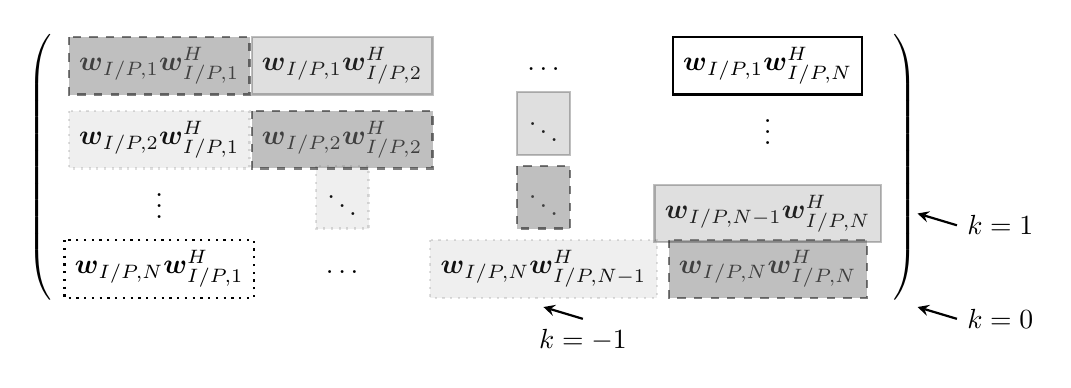
\begin{tikzpicture}[>=stealth,thick,baseline,every right delimiter/.append style={name=rd},]
							\matrix [matrix of math nodes,left delimiter=(,right delimiter=)] (m)
							{
								\boldsymbol{w}_{I/P,1}\boldsymbol{w}_{I/P,1}^H & \boldsymbol{w}_{I/P,1}\boldsymbol{w}_{I/P,2}^H & \dots & \boldsymbol{w}_{I/P,1}\boldsymbol{w}_{I/P,N}^H \\
								\boldsymbol{w}_{I/P,2}\boldsymbol{w}_{I/P,1}^H & \boldsymbol{w}_{I/P,2}\boldsymbol{w}_{I/P,2}^H & \ddots & \vdots \\
								\vdots & \ddots & \ddots & \boldsymbol{w}_{I/P,N-1}\boldsymbol{w}_{I/P,N}^H \\
								\boldsymbol{w}_{I/P,N}\boldsymbol{w}_{I/P,1}^H & \dots & \boldsymbol{w}_{I/P,N}\boldsymbol{w}_{I/P,N-1}^H & \boldsymbol{w}_{I/P,N}\boldsymbol{w}_{I/P,N}^H \\
							};
							\draw[dotted,thick] (m-4-1.north west) rectangle (m-4-1.south east);
							\draw[dotted,thick,fill=gray,opacity=0.125] (m-2-1.north west) rectangle (m-2-1.south east); \draw[dotted,thick,fill=gray,opacity=0.125] (m-3-2.north west) rectangle (m-3-2.south east); \draw[dotted,thick,fill=gray,opacity=0.125] (m-4-3.north west) rectangle (m-4-3.south east);
							\draw[dashed,thick,fill=gray,opacity=0.5] (m-1-1.north west) rectangle (m-1-1.south east); \draw[dashed,thick,fill=gray,opacity=0.5] (m-2-2.north west) rectangle (m-2-2.south east); \draw[dashed,thick,fill=gray,opacity=0.5] (m-3-3.north west) rectangle (m-3-3.south east); \draw[dashed,thick,fill=gray,opacity=0.5] (m-4-4.north west) rectangle (m-4-4.south east);
							\draw[solid,thick,fill=gray,opacity=0.25] (m-1-2.north west) rectangle (m-1-2.south east); \draw[solid,thick,fill=gray,opacity=0.25] (m-2-3.north west) rectangle (m-2-3.south east); \draw[solid,thick,fill=gray,opacity=0.25] (m-3-4.north west) rectangle (m-3-4.south east);
							\draw[solid,thick] (m-1-4.north west) rectangle (m-1-4.south east);
							\draw[<-] (m-4-3.south|-m.south) -- ++(0.5,-0.15) node[below]{$k=-1$};
							\draw[<-] (rd.east|-m.south) -- ++(0.5,-0.15) node[right]{$k=0$};
							\draw[<-] (rd.east|-m-3-4.east) -- ++(0.5,-0.15) node[right]{$k=1$};

						\end{tikzpicture}
				\end{equation*}
				\caption{$\boldsymbol{W}_{I/P}$ consists of $N \times N$ blocks of size $M \times M$. $\boldsymbol{W}_{I/P,k}$ keeps the $k$-th block diagonal of $\boldsymbol{W}_{I/P}$ and nulls all remaining blocks. Solid, dashed and dotted blocks correspond to $k>0$, $k=0$ and $k<0$, respectively. For $\boldsymbol{w}_{I/P,n_1}\boldsymbol{w}_{I/P,n_2}^H$, the $k$-th block diagonal satisfies $k=n_2-n_1$.}
				\label{fi:block_diagonal}
			\end{figure*}

			\begin{figure*}[b]
				\hrule
				\begin{equation}
					z(\boldsymbol{\phi},\boldsymbol{w}_I,\boldsymbol{w}_P,\rho) = \beta_2\rho\Bigl(\mathcal{E}\left\{\mathcal{A}\left\{y_{I}^2(t)\right\}\right\}+\mathcal{A}\left\{y_{P}^2(t)\right\}\Bigr)+\beta_4\rho^2\Bigl(\mathcal{E}\left\{\mathcal{A}\left\{y_{I}^4(t)\right\}\right\}+\mathcal{A}\left\{y_{P}^4(t)\right\}+6\mathcal{E}\left\{\mathcal{A}\left\{y_{I}^2(t)\right\}\right\}\mathcal{A}\left\{y_{P}^2(t)\right\}\Bigr)\,.\label{eq:z_expand}
				\end{equation}
				\hrule
				\begin{flalign}
					\mathcal{E}\left\{\mathcal{A}\left\{y_{I}^2(t)\right\}\right\}
					& = \frac{1}{2}\sum_{n=1}^N{(\boldsymbol{h}_{n}^H\boldsymbol{w}_{I,n})(\boldsymbol{h}_{n}^H\boldsymbol{w}_{I,n})^H} = \frac{1}{2}\boldsymbol{h}^H\boldsymbol{W}_{I,0}\boldsymbol{h}\,,&&\label{eq:y_I2}\\
					\mathcal{E}\left\{\mathcal{A}\left\{y_{I}^4(t)\right\}\right\}
					& = \frac{3}{4}\left(\sum_{n=1}^N{(\boldsymbol{h}_{n}^H\boldsymbol{w}_{I,n})(\boldsymbol{h}_{n}^H\boldsymbol{w}_{I,n})^H}\right)^2 = \frac{3}{4}(\boldsymbol{h}^H\boldsymbol{W}_{I,0}\boldsymbol{h})^2\,,&&\label{eq:y_I4}
				\end{flalign}
				\begin{align}
					\mathcal{A}\left\{y_{P}^2(t)\right\}
					& = \frac{1}{2}\sum_{n=1}^N{(\boldsymbol{h}_{n}^H\boldsymbol{w}_{P,n})(\boldsymbol{h}_{n}^H\boldsymbol{w}_{P,n})^H} = \frac{1}{2}\boldsymbol{h}^H\boldsymbol{W}_{P,0}\boldsymbol{h}\,,\label{eq:y_P2}\\
					\mathcal{A}\left\{y_{P}^4(t)\right\}
					& = \frac{3}{8}\sum_{\substack{{n_1},{n_2},{n_3},{n_4}\\{n_1}+{n_2}={n_3}+{n_4}}}{(\boldsymbol{h}_{{n_1}}^H\boldsymbol{w}_{P,{n_1}})(\boldsymbol{h}_{{n_2}}^H\boldsymbol{w}_{P,{n_2}})(\boldsymbol{h}_{{n_3}}^H\boldsymbol{w}_{P,{n_3}})^H(\boldsymbol{h}_{{n_4}}^H\boldsymbol{w}_{P,{n_4}})^H} = \frac{3}{8}\sum_{k=-N+1}^{N-1}(\boldsymbol{h}^H\boldsymbol{W}_{P,k}\boldsymbol{h})(\boldsymbol{h}^H\boldsymbol{W}_{P,k}\boldsymbol{h})^H\,.\label{eq:y_P4}
				\end{align}
			\end{figure*}
		\end{subsection}


		\begin{subsection}{Rate-Energy Region}
			The achievable R-E region is defined as
			\begin{align}
				C_{R_{\text{ID}}-I_{\text{EH}}}(P)
				&\triangleq \biggl\{(R_{\text{ID}}, I_{\text{EH}}): R_{\text{ID}} \le R, I_{\text{EH}} \le z,\nonumber\\
				&\quad \frac{1}{2}\left(\lVert{\boldsymbol{w}_I}\rVert^2+\lVert{\boldsymbol{w}_P}\rVert^2\right) \le P\biggr\}
			\end{align}
			where $P$ is the average transmit power budget and the coefficient \num{1/2} converts the peak power of sine waves to the average power.
		\end{subsection}
	\end{section}


	\begin{section}{Problem Formulation}\label{se:problem_formulation}
		We characterize the R-E region through a current maximization problem subject to transmit power, IRS magnitude, and rate constraints
		\begin{maxi!}
			{\boldsymbol{\phi},\boldsymbol{w}_I,\boldsymbol{w}_P,\rho}{z(\boldsymbol{\phi},\boldsymbol{w}_I,\boldsymbol{w}_P,\rho)}{\label{op:original}}{\label{ob:original}}
			\addConstraint{\frac{1}{2}\left(\lVert{\boldsymbol{w}_I}\rVert^2+\lVert{\boldsymbol{w}_P}\rVert^2\right)\le{P}}\label{co:original_power}
			\addConstraint{R(\boldsymbol{\phi},\boldsymbol{w}_I,\rho) \ge \bar{R}}\label{co:original_rate}
			\addConstraint{\lvert{\phi_l}\rvert=1, \quad l=1,\dots,L}\label{co:original_modulus}
			\addConstraint{0 \le \rho \le 1\,.}
		\end{maxi!}
		Problem~\eqref{op:original} is intricate as the variables are coupled and the objective function \eqref{ob:original}, the rate constraint \eqref{co:original_rate}, and the IRS magnitude constraint \eqref{co:original_modulus} are non-convex. To achieve a feasible solution, we propose an AO algorithm that iteratively updates the waveform and active beamforming at the transmitter, the phase shifts at the IRS, and the power splitting ratio at the receiver, until convergence.
		\begin{remark}\label{re:irs_subchannel_alignment}
			As information and power transfer prefer different subchannel strength distribution, the frequency-flat characteristic of the IRS introduces a resource allocation problem. Following Remark \ref{re:irs_frequency_flat}, if the IRS is frequency-selective and there is only one transmit antenna, then each reflector can simultaneously align the corresponding AP-IRS-user channel with the AP-user channel at all subbands. In this case, the strengths of all subchannels are maximized so that the joint design would follow straightforwardly from existing SWIPT work \cite{Clerckx2018b}.
		\end{remark}


		\begin{subsection}{IRS Phase Shift}
			In this section, the IRS phase shift $\boldsymbol{\phi}$ is optimized for any given waveform $\boldsymbol{w}_{I/P}$ and splitting ratio $\rho$. We observe that
			\begin{align}
				\lvert \boldsymbol{h}_{n}^H\boldsymbol{w}_{I,n} \rvert^2
				& = \boldsymbol{w}_{I,n}^H\boldsymbol{h}_n\boldsymbol{h}_n^H\boldsymbol{w}_{I,n}\nonumber\\
				& = \boldsymbol{w}_{I,n}^H(\boldsymbol{h}_{D,n}+\boldsymbol{V}_n^H\boldsymbol{\phi})(\boldsymbol{h}_{D,n}^H+\boldsymbol{\phi}^H\boldsymbol{V}_n)\boldsymbol{w}_{I,n}\nonumber\\
				& = \boldsymbol{w}_{I,n}^H\boldsymbol{M}_n^H\boldsymbol{\Phi}\boldsymbol{M}_n\boldsymbol{w}_{I,n}\nonumber\\
				& = \mathrm{Tr}(\boldsymbol{M}_n\boldsymbol{w}_{I,n}\boldsymbol{w}_{I,n}^H\boldsymbol{M}_n^H\boldsymbol{\Phi})\nonumber\\
				& = \mathrm{Tr}(\boldsymbol{C}_n\boldsymbol{\Phi})
			\end{align}
			where $t$ is an auxiliary variable with unit modulus, $\boldsymbol{M}_n=[\boldsymbol{V}_n^H, \boldsymbol{h}_{D,n}]^H \in \mathbb{C}^{(L+1) \times M}$, $\bar{\boldsymbol{\phi}}=[\boldsymbol{\phi}^H, t]^H \in \mathbb{C}^{(L+1) \times 1}$, $\boldsymbol{\Phi}=\bar{\boldsymbol{\phi}}\bar{\boldsymbol{\phi}}^H \in \mathbb{C}^{(L+1) \times (L+1)}$, $\boldsymbol{C}_n = \boldsymbol{M}_n\boldsymbol{w}_{I,n}\boldsymbol{w}_{I,n}^H\boldsymbol{M}_n^H \in \mathbb{C}^{(L+1)\times(L+1)}$. On the other hand, we define $t_{I/P,k}$ as
			\begin{align}
				t_{I/P,k}
				& = \boldsymbol{h}^H\boldsymbol{W}_{I/P,k}\boldsymbol{h}\nonumber\\
				& = \mathrm{Tr}(\boldsymbol{h}\boldsymbol{h}^H\boldsymbol{W}_{I/P,k})\nonumber\\
				& = \mathrm{Tr}\left((\boldsymbol{h}_{D}+\boldsymbol{V}^H\boldsymbol{\phi})(\boldsymbol{h}_{D}^H+\boldsymbol{\phi}^H\boldsymbol{V})\boldsymbol{W}_{I/P,k}\right)\nonumber\\
				& = \mathrm{Tr}(\boldsymbol{M}^H\boldsymbol{\Phi}\boldsymbol{M}\boldsymbol{W}_{I/P,k})\nonumber\\
				& = \mathrm{Tr}(\boldsymbol{M}\boldsymbol{W}_{I/P,k}\boldsymbol{M}^H\boldsymbol{\Phi})\nonumber\\
				& = \mathrm{Tr}(\boldsymbol{C}_{I/P,k}\boldsymbol{\Phi})
			\end{align}
			where $\boldsymbol{V}=[\boldsymbol{V}_1,\dots,\boldsymbol{V}_N] \in \mathbb{C}^{L \times MN}$, $\boldsymbol{M}=[\boldsymbol{V}^H, \boldsymbol{h}_{D}]^H \in \mathbb{C}^{(L+1) \times MN}$, $\boldsymbol{C}_{I/P,k}=\boldsymbol{M}\boldsymbol{W}_{I/P,k}\boldsymbol{M}^H \in \mathbb{C}^{(L+1)\times(L+1)}$. Therefore, we rewrite the rate and objective expressions as
			\begin{align}
				R(\boldsymbol{\Phi})
				& = \sum_{n=1}^{N}{\log_2\left(1+\frac{(1-\rho)\mathrm{Tr}(\boldsymbol{C}_n\boldsymbol{\Phi})}{\sigma_n^2}\right)}\,,\label{eq:R_irs}\\
				z(\boldsymbol{\Phi})
				& = \frac{1}{2}{\beta_2}{\rho}(t_{I,0}+t_{P,0})\nonumber\\
				& \quad + \frac{3}{8}{\beta_4}{\rho^2} \left(2t_{I,0}^2 + \sum_{k=-N+1}^{N-1}{t_{P,k}t_{P,k}^*}\right)\nonumber\\
				& \quad + \frac{3}{2}{\beta_4}{\rho^2}t_{I,0}t_{P,0}\,.\label{eq:z_irs}
			\end{align}
			To maximize non-concave expression \eqref{eq:z_irs}, we propose a SCA algorithm that approximate the second-order terms by first-order Taylor expansion \cite{Adali2010}. Based on the solution at iteration $i - 1$, the approximations at iteration $i$ are
			\begin{align}
				(t_{I,0}^{(i)})^2
				& \ge 2 t_{I,0}^{(i)}t_{I,0}^{(i-1)} - (t_{I,0}^{(i-1)})^2\,,\label{eq:taylor_1}\\
				t_{P,k}^{(i)} (t_{P,k}^{(i)})^*
				& \ge 2 \Re\left\{t_{P,k}^{(i)} (t_{P,k}^{(i-1)})^*\right\} - t_{P,k}^{(i-1)} (t_{P,k}^{(i-1)})^*\,,\label{eq:taylor_2}\\
				t_{I,0}^{(i)} t_{P,0}^{(i)}
				& = \frac{1}{4}(t_{I,0}^{(i)} + t_{P,0}^{(i)})^2 - \frac{1}{4}(t_{I,0}^{(i)} - t_{P,0}^{(i)})^2\nonumber\\
				& \ge \frac{1}{2}(t_{I,0}^{(i)} + t_{P,0}^{(i)})(t_{I,0}^{(i-1)} + t_{P,0}^{(i-1)})\nonumber\\
				& \quad - \frac{1}{4}(t_{I,0}^{(i-1)} + t_{P,0}^{(i-1)})^2 - \frac{1}{4}(t_{I,0}^{(i)} - t_{P,0}^{(i)})^2\label{eq:taylor_3}
			\end{align}
			which provide lower bounds to the corresponding terms in \eqref{eq:z_irs}. Hence, the objection function is approximated by $\tilde{z}(\boldsymbol{\Phi}^{(i)})$ in \eqref{eq:z_irs_approx}, and problem~\eqref{op:original} is transformed to
			\begin{figure*}[b]
				\hrule
				\begin{align}
					\tilde{z}(\boldsymbol{\Phi}^{(i)})
					& = \frac{1}{2}{\beta_2}{\rho}(t_{I,0}^{(i)}+t_{P,0}^{(i)})\nonumber\\
					& \quad + \frac{3}{8}{\beta_4}{\rho^2} \left(4 (t_{I,0}^{(i)})(t_{I,0}^{(i-1)}) - 2 (t_{I,0}^{(i-1)})^2 + \sum_{k=-N+1}^{N-1}{2 \Re\left\{t_{P,k}^{(i)} (t_{P,k}^{(i-1)})^*\right\} - t_{P,k}^{(i-1)} (t_{P,k}^{(i-1)})^*}\right)\nonumber\\
					& \quad + \frac{3}{2}{\beta_4}{\rho^2} \left(\frac{1}{2}(t_{I,0}^{(i)} + t_{P,0}^{(i)})(t_{I,0}^{(i-1)} + t_{P,0}^{(i-1)}) - \frac{1}{4}(t_{I,0}^{(i-1)} + t_{P,0}^{(i-1)})^2 - \frac{1}{4}(t_{I,0}^{(i)} - t_{P,0}^{(i)})^2\right)\,.\label{eq:z_irs_approx}
				\end{align}
			\end{figure*}
			\begin{maxi!}
				{\boldsymbol{\Phi}}{\tilde{z}(\boldsymbol{\Phi})}{\label{op:irs}}{\label{ob:irs}}
				\addConstraint{R(\boldsymbol{\Phi}) \ge \bar{R}}\label{co:irs_rate}
				\addConstraint{\boldsymbol{\Phi}_{l,l}=1, \quad l=1,\dots,L+1}\label{co:irs_modulus}
				\addConstraint{\boldsymbol{\Phi}\succeq{0}}
				\addConstraint{\mathrm{rank}(\boldsymbol{\Phi})=1\,.\label{co:irs_rank}}
			\end{maxi!}
			Problem~\eqref{op:irs} is not a standard Semidefinite Programming (SDP). If we relax the rank constraint \eqref{co:irs_rank} to formulate a convex problem, there is no guarantee $\boldsymbol{\Phi}^{\star}$ is rank-\num{1}, and the optimal rank-\num{1} solution $\bar{\boldsymbol{\phi}}^{\star}$ extracted from $\boldsymbol{\Phi}^{\star}$ may not be a stationary point of the original problem~\eqref{op:original}. In Section~\ref{se:performance_evaluation}, we numerically show that $\boldsymbol{\Phi}^{\star}$ is rank-\num{1} for all tested channel realizations under different configurations such that the performance loss by SDR is insignificant. Problem~\eqref{op:irs} without constraint \ref{co:irs_rank} can be solved using existing optimization tools such as CVX \cite{Grant2013}.

			When $\boldsymbol{\Phi}^{\star}$ is rank-\num{1}, the optimal phase shift vector $\bar{\boldsymbol{\phi}}^\star$ can be obtained by Eigenvalue Decomposition (EVD). Otherwise, a suboptimal solution can be extracted via Gaussian randomization method \cite{Huang2010}. Specifically, we perform EVD $\boldsymbol{\Phi}^{\star}=\boldsymbol{U}\boldsymbol{\Sigma}\boldsymbol{U}^H$, generate $Q$ CSCG random vectors $\boldsymbol{r}_q \sim \mathcal{CN}(\boldsymbol{0},\boldsymbol{I}_{L+1}),\ q=1,\dots,Q$, construct the corresponding candidates $\bar{\boldsymbol{\phi}}_q=e^{j\arg\left(\boldsymbol{U}\boldsymbol{\Sigma}^{1/2}\boldsymbol{r}_q\right)}$, and choose the one that maximizes the objective function \eqref{ob:irs}. Finally, the phase shifts are retrieved by $\theta_l^{\star}=\arg(\phi_l^\star/\phi_{L+1}^\star), \ l=1,\dots,L$. The SCA algorithm for passive beamforming optimization is summarized in Algorithm~\ref{al:irs}.
			\begin{algorithm}[!t]
				\caption{SCA: IRS Phase Shift.}
				\label{al:irs}
				\begin{algorithmic}[1]
					\State \textbf{input} $\beta_2,\beta_4,\boldsymbol{h}_{D,n},\boldsymbol{H}_{I,n},\boldsymbol{h}_{R,n},\boldsymbol{w}_I,\boldsymbol{w}_P,\rho,\sigma_n,\bar{R},Q,\epsilon$
					\State Construct $\boldsymbol{M},\boldsymbol{M}_n,\boldsymbol{C}_{n}$, $\boldsymbol{C}_{I/P,k}$, $\forall n,k$
					\State \textbf{initialize} $i \gets 0,\boldsymbol{\Phi}^{(0)},t_{I/P,k}^{(0)}, \forall k$
					\Repeat
						\State $i \gets i + 1$
						\State Obtain $\boldsymbol{\Phi}^{(i)}, t_{I/P,k}^{(i)}$ by solving problem~\eqref{op:irs}
						\State Compute $z^{(i)}$ by \eqref{eq:z_irs}
					\Until $\lvert z^{(i)}-z^{(i-1)} \rvert \le \epsilon$
					\State Set $\boldsymbol{\Phi}^{\star}=\boldsymbol{\Phi}^{(i)}$
					\If{$\mathrm{rank}(\boldsymbol{\Phi}^{\star})=1$}
						\State Obtain $\bar{\boldsymbol{\phi}}^\star$ by EVD, $\boldsymbol{\Phi}^{\star}=\bar{\boldsymbol{\phi}}^\star(\bar{\boldsymbol{\phi}}^\star)^H$
					\Else
						\State Obtain $\boldsymbol{U},\boldsymbol{\Sigma}$ by EVD, $\boldsymbol{\Phi}^{\star}=\boldsymbol{U}\boldsymbol{\Sigma}\boldsymbol{U}^H$
						\State Generate $\boldsymbol{r}_q \sim \mathcal{CN}(\boldsymbol{0},\boldsymbol{I}_{L+1})$, $q=1,\dots,Q$
						\State Construct $\bar{\boldsymbol{\phi}}_q=e^{j\arg\left(\boldsymbol{U}\boldsymbol{\Sigma}^{1/2}\boldsymbol{r}_q\right)}$, $\boldsymbol{\Phi}_q=\bar{\boldsymbol{\phi}}_q\bar{\boldsymbol{\phi}}_q^H$
						\State Set $q^{\star}=\arg\max_q{z(\boldsymbol{\Phi}_q)}$, $\bar{\boldsymbol{\phi}}^\star=\bar{\boldsymbol{\phi}}_{q^{\star}}$
					\EndIf
					\State Set $\theta_l^\star=\arg(\phi_l^\star/\phi_{L+1}^\star), \ l=1,\dots,L$, and construct $\boldsymbol{\phi}^{\star}$
					\State \textbf{output} $\boldsymbol{\phi}^{\star}$
				\end{algorithmic}
			\end{algorithm}
		\end{subsection}


		\begin{subsection}{Waveform and Splitting Ratio}
			Next, we jointly optimize both information and power waveforms $\boldsymbol{w}_{I/P}$ together with splitting ratio $\rho$ for any given IRS phase shift $\boldsymbol{\phi}$. As pointed out in \cite{Clerckx2018b}, the waveform design in frequency and spatial domain can be decoupled without performance loss, and the optimal spatial weight is given by Maximum-Ratio Transmission (MRT) beamformer
			\begin{equation}\label{eq:w_IP}
				\boldsymbol{w}_{I/P,n}=s_{I/P,n}\frac{\boldsymbol{h}_n}{\lVert{\boldsymbol{h}_n}\rVert}\,.
			\end{equation}
			That is to say, for single-user MISO SWIPT, the optimal active beamformer is MRT and we only need to determine the amplitudes $s_{I/P,n}$ at different tones. Hence, the original waveform optimization with $2MN$ complex variables is converted into a power allocation problem with $2N$ nonnegative real variables. Let $\boldsymbol{s}_{I/P}=[s_{I/P,1},\dots,s_{I/P,N}]^T \in \mathbb{C}^{N \times 1}$. At subband $n$, the effective channel gain is given by $\lVert{\boldsymbol{h}_n}\rVert$, and the power allocated to the modulated and unmodulated waveform are given by $s_{I,n}^2$ and $s_{P,n}^2$, respectively. With such an active beamformer selection, we have $\boldsymbol{h}_n^H\boldsymbol{w}_{I,n}=\lvert{\boldsymbol{h}_n^H\boldsymbol{w}_{I,n}}\rvert=\lVert{\boldsymbol{h}_n}\rVert s_{I,n}$ such that the rate and objective functions further reduce to \eqref{eq:R_waveform} and \eqref{eq:z_waveform}, respectively.
			\begin{equation}\label{eq:R_waveform}
				R(\boldsymbol{s}_I,\rho) = \log_2\left(\prod_{n=1}^N\biggl(1+\frac{(1-\rho)\lVert{\boldsymbol{h}_n}\rVert^2 s_{I,n}^2}{\sigma_n^2}\biggr)\right)\,.
			\end{equation}
			\begin{figure*}[b]
				\hrule
				\begin{align}
					z(\boldsymbol{s}_I,\boldsymbol{s}_P,\rho)
					& = \frac{1}{2}{\beta_2}{\rho} \sum_{n=1}^N \lVert{\boldsymbol{h}_n}\rVert^2(s_{I,n}^2+s_{P,n}^2)\nonumber\\
					& \quad + \frac{3}{8}{\beta_4}{\rho^2} \left( 2\sum_{n_1,n_2} \prod_{j=1}^2 \lVert{\boldsymbol{h}_{n_j}}\rVert^2 s_{I,{n_j}}^2 + \sum_{\substack{{n_1},{n_2},{n_3},{n_4}\\{n_1}+{n_2}={n_3}+{n_4}}} \prod_{j=1}^4 \lVert{\boldsymbol{h}_{n_j}}\rVert s_{P,{n_j}} \right)\nonumber\\
					& \quad + \frac{3}{2}{\beta_4}{\rho^2} \left( \sum_{n_1,n_2} \lVert{\boldsymbol{h}_{n_1}}\rVert^2 \lVert{\boldsymbol{h}_{n_2}}\rVert^2 s_{I,{n_1}}^2 s_{P,{n_2}}^2 \right)\,.\label{eq:z_waveform}
				\end{align}
			\end{figure*}%
			Therefore, problem~\eqref{op:original} is reduced to an amplitude optimization issue
			\begin{maxi!}
				{\boldsymbol{s}_I,\boldsymbol{s}_P,\rho}{z(\boldsymbol{s}_I,\boldsymbol{s}_P,\rho)}{\label{op:waveform}}{}
				\addConstraint{\frac{1}{2}\left(\lVert{\boldsymbol{s}_I}\rVert^2+\lVert{\boldsymbol{s}_P}\rVert^2\right)\le{P}}
				\addConstraint{R(\boldsymbol{s}_I,\rho) \ge \bar{R}\,.}
			\end{maxi!}
			Since problem~\eqref{op:waveform} involves the production of nonnegative real variables, we introduce auxiliary variables $t',\bar{\rho}$ and transform it into a reversed GP
			\begin{mini!}
				{\boldsymbol{s}_I,\boldsymbol{s}_P,\rho,\bar{\rho},t'}{\frac{1}{t'}}{\label{op:waveform_rgp}}{}
				\addConstraint{\frac{1}{2}\left(\lVert{\boldsymbol{s}_I}\rVert^2+\lVert{\boldsymbol{s}_P}\rVert^2\right) \le P}\label{co:waveform_power}
				\addConstraint{\frac{t'}{z(\boldsymbol{s}_I,\boldsymbol{s}_P,\rho)} \le 1}\label{co:waveform_objective}
				\addConstraint{\frac{2^{\bar{R}}}{\prod_{n=1}^N \left(1+{\bar{\rho}\lVert{\boldsymbol{h}_n}\rVert^2 s_{I,n}^2}\big/{\sigma_n^2}\right)} \le 1}\label{co:waveform_rate}
				\addConstraint{\rho + \bar{\rho} \le 1\,.}
			\end{mini!}
			The denominators of \eqref{co:waveform_objective}, \eqref{co:waveform_rate} are posynomials \cite{Boyd2007} that are further decomposed as
			\begin{align}
				z(\boldsymbol{s}_I,\boldsymbol{s}_P,\rho)&=\sum_{m_P}{g_{m_P}(\boldsymbol{s}_I,\boldsymbol{s}_P,\rho)}\label{eq:posynomial_objective}\,,\\
				1+\frac{\bar{\rho}\lVert{\boldsymbol{h}_n}\rVert^2 s_{I,n}^2}{\sigma_n^2}&=\sum_{m_{I,n}}g_{m_{I,n}}(s_{I,n},\bar{\rho})\label{eq:posynomial_rate}
			\end{align}
			where $m_P=(2N^3+6N^2+7N)/3$, $m_{I,n}=2$ are the number of monomials. Following \cite{Chiang2005}, we upper bound posynomials \eqref{eq:posynomial_objective} and \eqref{eq:posynomial_rate} by Arithmetic Mean-Geometric Mean (AM-GM) inequality such that problem~\eqref{op:waveform_rgp} reduces to
			\begin{mini!}
				{\boldsymbol{s}_I,\boldsymbol{s}_P,\rho,\bar{\rho},t'}{\frac{1}{t'}}{\label{op:waveform_gp}}{}
				\addConstraint{\frac{1}{2}\left(\lVert{\boldsymbol{s}_I}\rVert^2+\lVert{\boldsymbol{s}_P}\rVert^2\right)\le{P}}
				\addConstraint{{t'}\prod_{m_P}{\left(\frac{g_{{m_P}}(\boldsymbol{s}_I,\boldsymbol{s}_P,\rho)}{\gamma_{{m_P}}}\right)^{-\gamma_{{m_P}}}}\le{1}}
				\addConstraint{2^{\bar{R}}\prod_{n}\prod_{m_{I,n}}\left(\frac{g_{m_{I,n}}(s_{I,n},\bar{\rho})}{\gamma_{m_{I,n}}}\right)^{-\gamma_{m_{I,n}}}\le{1}}
				\addConstraint{\rho + \bar{\rho} \le 1}
			\end{mini!}
			where $\gamma_{m_P},\gamma_{m_{I,n}} \ge 0$, $\sum_{m_P}\gamma_{m_P}=\sum_{m_{I,n}}\gamma_{m_{I,n}}=1$. The tightness of the AM-GM inequality depends on $\{\gamma_{m_P},\gamma_{m_{I,n}}\}$ that require successive update. As suggested in \cite{Clerckx2018b}, a feasible choice at iteration $i$ is
			\begin{align}
				\gamma_{m_P}^{(i)} & = \frac{g_{m_P}(\boldsymbol{s}_I^{(i-1)},\boldsymbol{s}_P^{(i-1)},\rho^{(i-1)})}{z(\boldsymbol{s}_I^{(i-1)},\boldsymbol{s}_P^{(i-1)},\rho^{(i-1)})}\label{eq:gamma_P}\,,\\
				\gamma_{m_{I,n}}^{(i)} & = \frac{g_{m_{I,n}}(s_{I,n}^{(i-1)},\bar{\rho}^{(i-1)})}{1+{\bar{\rho}^{(i-1)}\lVert{\boldsymbol{h}_n}\rVert^2 (s_{I,n}^{(i-1)})^2}\big/{\sigma_n^2}}\,.\label{eq:gamma_I}
			\end{align}
			Problem~\eqref{op:waveform_gp} can be solved using existing optimization tools such as CVX \cite{Grant2013}. $\boldsymbol{s}_I,\boldsymbol{s}_P,\rho$ are updated iteratively until convergence. The GP algorithm of waveform, active beamforming and splitting ratio optimization is summarized in Algorithm~\ref{al:waveform}.
			\begin{algorithm}[!t]
				\caption{GP: Waveform, Active Beamforming and Splitting Ratio.}
				\label{al:waveform}
				\begin{algorithmic}[1]
					\State \textbf{input} $\beta_2,\beta_4,\boldsymbol{h},P,\sigma_n,\bar{R},\epsilon$
					\State \textbf{initialize} $i \gets 0$, $\boldsymbol{s}_{I/P}^{(0)}$, $\rho^{(0)}$
					\Repeat
						\State $i \gets i + 1$
						\State Update $\{\gamma_{m_P}^{(i)},\gamma_{m_{I,n}}^{(i)}\}$ by \eqref{eq:gamma_P}, \eqref{eq:gamma_I}
						\State Obtain $\boldsymbol{s}_{I/P}^{(i)},\rho^{(i)}$ by solving problem~\eqref{op:waveform_gp}
						\State Compute $z^{(i)}$ by \eqref{eq:z_waveform}
					\Until $\lvert z^{(i)} - z^{(i-1)} \rvert \le \epsilon$
					\State Set $\boldsymbol{s}_{I/P}^{\star}=\boldsymbol{s}_{I/P}^{(i)}$, $\rho^{\star}=\rho^{(i)}$, retrieve $\boldsymbol{w}_{I/P}^{\star}$ by \eqref{eq:w_IP}
					\State \textbf{output} $\boldsymbol{w}_{I/P}^{\star}, \rho^{\star}$
				\end{algorithmic}
			\end{algorithm}
		\end{subsection}


		\begin{subsection}{Alternating Optimization}
			For any direct, incident and reflective channels, we iteratively update the passive beamforming by Algorithm~\ref{al:irs}, and waveform, active beamforming and splitting ratio by Algorithm~\ref{al:waveform} until convergence. The AO algorithm is summarized in Algorithm~\ref{al:alternating}.
			\begin{algorithm}[!t]
				\caption{AO: Waveform, Active and Passive Beamforming.}
				\label{al:alternating}
				\begin{algorithmic}[1]
					\State \textbf{input} $\beta_2,\beta_4,\boldsymbol{h}_{D,n},\boldsymbol{H}_{I,n},\boldsymbol{h}_{R,n},P,\sigma_n,\bar{R},Q,\epsilon$
					\State \textbf{initialize} $i \gets 0$, $\boldsymbol{\phi}^{(0)},\boldsymbol{w}_{I/P}^{(0)},\rho^{(0)}$
					\Repeat
						\State $i \gets i + 1$
						\State Fix $\boldsymbol{w}_{I/P}^{(i-1)},\rho^{(i-1)}$ and obtain $\boldsymbol{\phi}^{(i)}$ by Algorithm~\ref{al:irs}
						\State Fix $\boldsymbol{\phi}^{(i)}$, update $\boldsymbol{h}_n^{(i)}$ by \eqref{eq:h_n}, and obtain $\boldsymbol{w}_{I/P}^{(i)}, \rho^{(i)}$ by Algorithm~\ref{al:waveform}
						\State Compute $z^{(i)}$ by \eqref{eq:z_irs}
					\Until $\lvert z^{(i)} - z^{(i-1)} \rvert \le \epsilon$
					\State \textbf{output} $\boldsymbol{\phi}^{\star}, \boldsymbol{w}_{I/P}^{\star}, \rho^{\star}$
				\end{algorithmic}
			\end{algorithm}
		\end{subsection}


		\begin{subsection}{Convergence}
			\begin{proposition}\label{pr:irs}
				For any feasible initial point, the proposed SCA-based Algorithm~\ref{al:irs} can provide a feasible $\boldsymbol{\Phi}^{\star}$ that satisfies the KKT conditions, although there is no guarantee $\boldsymbol{\Phi}^{\star}$ is rank-\num{1}.
			\end{proposition}

			\begin{proof}\label{pf:irs}
				The objective function \eqref{ob:irs} is non-decreasing over iterations because the solution of problem~\eqref{op:irs} at iteration $i-1$ is still a feasible point at iteration $i$. Moreover, the sequence $\{\tilde{z}(\boldsymbol{\Phi}^{(i)})\}_{i=1}^{\infty}$ is bounded above due to the unit-modulus constraint \eqref{co:irs_modulus}. Thus, Algorithm~\ref{al:irs} is guaranteed to converge. To prove $\boldsymbol{\Phi}^{(i)}$ converges to the set of stationary points of IRS subproblem, we notice that the SCA-based Algorithm~\ref{al:irs} is indeed an inner approximation algorithm \cite{Marks1978}, since $\tilde{z}(\boldsymbol{\Phi}) \le z(\boldsymbol{\Phi})$, $\partial\tilde{z}(\boldsymbol{\Phi}^{(i)})/\partial\boldsymbol{\Phi}=\partial z(\boldsymbol{\Phi}^{(i)})/\partial\boldsymbol{\Phi}$ and the approximation \eqref{eq:taylor_1} -- \eqref{eq:taylor_3} are asymptotically tight as $i \to \infty$ \cite{Li2013}. Therefore, Algorithm~\ref{al:irs} is guaranteed to provide a feasible $\boldsymbol{\Phi}^{\star}$ that satisfies the KKT conditions.
			\end{proof}

			\begin{proposition}\label{pr:waveform}
				For any feasible initial point, the GP-based Algorithm~\ref{al:waveform} is guaranteed to converge to a stationary point of the waveform and splitting ratio subproblem.
			\end{proposition}

			\begin{proof}\label{pf:waveform}
				See \cite{Clerckx2016a,Clerckx2018b}.
			\end{proof}

			\begin{proposition}\label{pr:ao}
				Suppose $\boldsymbol{\Phi}$ is rank-\num{1}, every limit point $(\boldsymbol{\phi}^{\star},\boldsymbol{w}_I^{\star},\boldsymbol{w}_P^{\star},\rho^{\star})$ of the proposed alternating algorithm is a stationary point of the original problem~\eqref{op:original}.
			\end{proposition}

			\begin{proof}\label{pf:ao}
				The objective function \eqref{ob:original} is non-decreasing over iterations of Algorithm~\ref{al:alternating}, which is also upper-bounded due to the unit-modulus constraint \eqref{co:original_modulus} and the average transmit power constraint \eqref{co:original_power}. If $\boldsymbol{\Phi}$ is rank-\num{1}, then $\boldsymbol{\phi}$ can be obtained by EVD without performance loss, and the sequence $\{\boldsymbol{\phi}^{(i)},\boldsymbol{w}_I^{(i)},\boldsymbol{w}_P^{(i)},\rho^{(i)}\}$ generated by alternatively optimizing $\boldsymbol{\phi}$ and $\boldsymbol{w}_I,\boldsymbol{w}_P,\rho$ has limit points so that Algorithm~\ref{al:alternating} is guaranteed to converge. As demonstrated in \cite{Grippo2000}, the solution is a stationary point of problem~\eqref{op:original}.
			\end{proof}
		\end{subsection}
	\end{section}


	\begin{section}{Performance Evaluations}\label{se:performance_evaluation}
		\begin{figure}[!t]
			\centering
			\def\svgwidth{\columnwidth}
			\import{assets/}{layout.pdf_tex}
			\caption{System layout in the simulation.}
			\label{fi:layout}
		\end{figure}
		To evaluate the performance of the proposed IRS-aided SWIPT system, we characterize the average R-E regions under typical setups. Consider a large open space WiFi-like environment at a center frequency of \SI{5.18}{\GHz} with reference bandwidth $B=1\,\si{\MHz}$. As shown in Fig.~\ref{fi:layout}, we assume the IRS moves along a horizontal line parallel to the AP-user path and let $d_H$, $d_V$ be the horizontal and vertical distances from the AP to the IRS, respectively. We also denote $d_D$, $d_I$, $d_R$ as the length of direct, incident, reflective paths such that $d_I=\sqrt{d_H^2+d_V^2}$, $d_R=\sqrt{(d_D-d_H)^2+d_V^2}$. We choose as reference $d_D=15\,\si{\meter}$, $d_V=2\,\si{\meter}$ and $d_H=2\,\si{\meter}$. The path loss and fading parameters are obtained from IEEE TGn channel model D \cite{Erceg2004}, and reference path loss is set to $L_0=-35\,\si{\dB}$ at $d_0=1\,\si{\meter}$. We assume all channels are NLoS with taps modelled as i.i.d. CSCG random variables of unit average sum-power to create a normalized multipath response. The reference numbers of transmit antennas, IRS reflectors and subbands are $M=1$, $L=20$, $N=16$, respectively. No spatial correlation is considered across transmit antennas and IRS arrays. Rectenna parameters are taken as $k_2=0.0034$, $k_4=0.3829$, $R_{\text{ant}}=50\,\si{\ohm}$. With \SI{0}{\dBi} transmit antenna gain, the average Effective Isotropic Radiated Power (EIRP) is fixed to $P=36\,\si{\dBm}$ while the reference average noise power is $\sigma_n=-40\,\si{\dBm}$ at all subbands. We also assume \SI{0}{\dBi} IRS element gain and \SI{2}{\dBi} receive antenna gain. For the algorithm, the tolerance is $\epsilon=10^{-8}$, the number of candidates in the Gaussian randomization method is $Q=10^{3}$, and the R-E region is averaged over \num{200} channel realizations. In the R-E boundary, the leftmost point corresponds to WPT ($\rho=1$) where power can be allocated simultaneously to modulated and unmodulated waveform to maximize the average output DC current.
		% - at the WPT point, power is allocated to the multisine waveform only, isn't it?
		% - for single-carrier WPT, modulated waveform may be preferred as it has a modulation gain (also proved in Fig. 5)
		On the other hand, the rightmost point corresponds to WIT ($\rho=0$) where the solution coincides with the Water-Filling (WF) algorithm that allocates all power to modulated waveform only. For a fair comparison, the $x$-axis of the plots has been normalized to the average subband rate $R/N$.

		We first evaluate the performance of Algorithm~\ref{al:irs} under SDR. It is demonstrated that $\boldsymbol{\Phi}^{\star}$ is rank-\num{1} for all tested channel realizations with different $M$, $N$ and $L$. Therefore, $\boldsymbol{\phi}^{\star}$ can be directly obtained through EVD and we claim Algorithm~\ref{al:irs} converges to stationary points of problem~\eqref{op:irs} without performance loss.

		\begin{figure}[!t]
			\centering
			\begin{adjustbox}{width=\linewidth}
				% This file was created by matlab2tikz.
%
%The latest updates can be retrieved from
%  http://www.mathworks.com/matlabcentral/fileexchange/22022-matlab2tikz-matlab2tikz
%where you can also make suggestions and rate matlab2tikz.
%
\definecolor{mycolor1}{rgb}{0.00000,0.44700,0.74100}%
\definecolor{mycolor2}{rgb}{0.85000,0.32500,0.09800}%
\definecolor{mycolor3}{rgb}{0.92900,0.69400,0.12500}%
\definecolor{mycolor4}{rgb}{0.49400,0.18400,0.55600}%
\definecolor{mycolor5}{rgb}{0.46600,0.67400,0.18800}%
%
\begin{tikzpicture}

\begin{axis}[%
width=4.036in,
height=3.396in,
at={(0.677in,0.458in)},
scale only axis,
xmin=0,
xlabel style={font=\color{white!15!black}},
xlabel={Per-subband rate [bps/Hz]},
ymin=0,
ylabel style={font=\color{white!15!black}},
ylabel={DC current [$\mu$A]},
axis background/.style={fill=white},
xmajorgrids,
ymajorgrids,
legend style={legend cell align=left, align=left, draw=white!15!black},
title style={font=\huge}, label style={font=\huge}, ticklabel style={font=\LARGE}, legend style={font=\LARGE}
]
\addplot [color=mycolor1, line width=2.0pt, mark=o, mark options={solid, mycolor1}]
  table[row sep=crcr]{%
10.4735835230447	2.22044604925031e-10\\
9.92234228501261	9.32112444582221\\
9.37110104856655	19.9734884440997\\
8.81985981522077	28.9045803554951\\
8.2686185819348	35.6026963553208\\
7.71737734737495	40.3640298249635\\
7.16613611329223	43.6515839749441\\
6.61489489962449	45.8838384219186\\
6.06365369435709	47.3846143361325\\
5.51241254125065	48.387712164817\\
4.96117133174749	49.0559031374681\\
4.40993010758737	49.5001897756857\\
3.85868881960391	49.7953550653237\\
3.30744769321745	49.9914147827456\\
2.75620680490471	50.1216779322935\\
2.20496539207832	50.2082717407884\\
1.65372490382178	50.2658783675822\\
1.10248502521887	50.3042351384749\\
0.551244201798665	50.3297984304523\\
0.00208272021122725	50.3468032636274\\
};
\addlegendentry{PS: $N = 1$}

\addplot [color=mycolor2, dashed, line width=2.0pt, mark=+, mark options={solid, mycolor2}]
  table[row sep=crcr]{%
9.46439299472766	2.22044604925031e-10\\
8.96626704732983	8.33259901113237\\
8.46814110217854	18.1592467782588\\
7.97001516810678	26.8459057443986\\
7.47188927991203	33.7865884977658\\
6.97376349389734	39.1021182696728\\
6.47563788783726	43.1095734137526\\
5.97751254554593	46.1263254362014\\
5.47938759571205	48.4100924422181\\
4.9812631417132	50.1570422133681\\
4.48313986198878	51.5129653769659\\
3.9850184151061	52.5860764238752\\
3.48690223959099	53.4644932017907\\
2.98881625901995	54.2152907388071\\
2.4907686856515	54.876350519767\\
1.9927085816719	55.4102601313978\\
1.49452596230085	55.7507587808269\\
0.996328503800862	55.9228678945531\\
0.498155311937769	56.0050195327705\\
7.96561638833979e-05	56.0440908160315\\
};
\addlegendentry{PS: $N = 2$}

\addplot [color=mycolor3, dotted, line width=2.0pt, mark=square, mark options={solid, mycolor3}]
  table[row sep=crcr]{%
8.46474130881161	2.22044604925031e-10\\
8.01922860825854	7.39556637278252\\
7.57371590798923	16.3301528528171\\
7.12820320923384	24.5530578014679\\
6.68269051784111	31.4067581548414\\
6.23717784712245	36.8807723848698\\
5.79166520659193	41.1848071966103\\
5.34615260904505	44.5637479552436\\
4.90064005868852	47.1819433421252\\
4.45512758053841	49.3115311617719\\
4.00961529688703	51.3192185929736\\
3.56410368036957	53.2799509313977\\
3.11859313382213	55.1790392738117\\
2.67308213993358	56.9434910638753\\
2.22757389355969	58.5545320511613\\
1.78206849076881	60.0507071304301\\
1.33656667993295	61.4246520887733\\
0.891059451890333	62.6856916109175\\
0.445528410592004	63.8224278268673\\
4.27142625741546e-05	65.7566997793879\\
};
\addlegendentry{PS: $N = 4$}

\addplot [color=mycolor4, dashdotted, line width=2.0pt, mark=x, mark options={solid, mycolor4}]
  table[row sep=crcr]{%
7.46967940598189	2.22044604925031e-10\\
7.07653838451426	6.48656081362313\\
6.68339736333032	14.4878192539044\\
6.29025634335385	22.1341941957671\\
5.8971153297914	28.7620953682232\\
5.50397433634409	34.2556110325877\\
5.1108333712231	38.6596718267908\\
4.71769245694479	43.72458608339\\
4.32455161953019	49.7166591178922\\
3.93141094330047	55.9262863516291\\
3.538270573739	62.0278844197607\\
3.14513042203963	67.9449898452885\\
2.75198993284372	73.575047324874\\
2.35884923255337	78.8756358471696\\
1.96571038246792	83.8429146410052\\
1.57257239299274	88.5577609221184\\
1.17943327753835	93.0781801797417\\
0.786298797114347	97.5891822379031\\
0.39317423652411	102.498290892545\\
6.66593915196139e-06	111.936209650345\\
};
\addlegendentry{PS: $N = 8$}

\addplot [color=mycolor5, line width=2.0pt, mark=triangle, mark options={solid, mycolor5}]
  table[row sep=crcr]{%
6.48048278576575	2.22044604925031e-10\\
6.13940474426762	5.60700734642188\\
5.7983267030979	12.647234679346\\
5.45724866316513	19.6236562694278\\
5.11617062902079	25.8031593109154\\
4.77509261174701	31.7417039076399\\
4.43401464078316	40.1213288425821\\
4.0929368009742	50.3041581039783\\
3.75185917286373	61.5535748607958\\
3.41078168220348	73.3823341604998\\
3.06970396145884	85.4598577072889\\
2.72862623901636	97.5503801097975\\
2.38754804867769	109.47814361271\\
2.04647081806535	121.155633291461\\
1.70539518844927	132.568113582494\\
1.36431849072778	143.792275087475\\
1.02324491987972	155.013982363149\\
0.682176465013792	166.662644650854\\
0.341113017781466	179.912499533855\\
2.61269538646837e-08	207.256703045906\\
};
\addlegendentry{PS: $N = 16$}

\addplot [color=red, dashed, line width=2.0pt, mark=triangle, mark options={solid, rotate=180, red}]
  table[row sep=crcr]{%
7.46967940598189	2.22044604925031e-10\\
6.29025634335385	22.1341941957671\\
5.8971153297914	28.7620953682232\\
2.75198993284372	73.575047324874\\
6.66593915196139e-06	111.936209650345\\
};
\addlegendentry{TS + PS: $N = 8$}

\addplot [color=black, dotted, line width=2.0pt, mark=triangle, mark options={solid, rotate=270, black}]
  table[row sep=crcr]{%
2.61269538646837e-08	207.256703045906\\
6.48048278576575	2.22044604925031e-10\\
};
\addlegendentry{TS: $N = 16$}

\end{axis}
\end{tikzpicture}%
			\end{adjustbox}
			\caption{Average R-E region versus $N$ for $M=1$, $L=20$, $\sigma_n=-40\,\si{\dBm}$, $B=1\,\si{\MHz}$ and $d_H=d_V=2\,\si{\meter}$.}
			\label{fi:re_subband}
		\end{figure}

		\begin{figure}[!t]
			\centering
			\begin{adjustbox}{width=\linewidth}
				% This file was created by matlab2tikz.
%
%The latest updates can be retrieved from
%  http://www.mathworks.com/matlabcentral/fileexchange/22022-matlab2tikz-matlab2tikz
%where you can also make suggestions and rate matlab2tikz.
%
\definecolor{mycolor1}{rgb}{0.00000,0.44700,0.74100}%
\definecolor{mycolor2}{rgb}{0.85000,0.32500,0.09800}%
%
\begin{tikzpicture}

\begin{axis}[%
width=4.521in,
height=0.544in,
at={(0.758in,3.503in)},
scale only axis,
xmin=0,
xmax=2,
xtick={1},
ymin=0,
axis background/.style={fill=white},
xmajorgrids,
ymajorgrids,
legend style={legend cell align=left, align=left, draw=white!15!black}
]
\addplot[ycomb, color=mycolor1, line width=2.0pt, mark=o, mark options={solid, mycolor1}] table[row sep=crcr] {%
1	2.5413547897652\\
};
\addplot[forget plot, color=white!15!black, line width=2.0pt] table[row sep=crcr] {%
0	0\\
2	0\\
};
\addlegendentry{$s_I$}

\addplot[ycomb, color=mycolor2, line width=2.0pt, mark=x, mark options={solid, mycolor2}] table[row sep=crcr] {%
1	1.17726395475229\\
};
\addplot[forget plot, color=white!15!black, line width=2.0pt] table[row sep=crcr] {%
0	0\\
2	0\\
};
\addlegendentry{$s_P$}

\end{axis}

\begin{axis}[%
width=4.521in,
height=0.544in,
at={(0.758in,2.747in)},
scale only axis,
xmin=0,
xmax=3,
xtick={1, 2},
ymin=0,
axis background/.style={fill=white},
xmajorgrids,
ymajorgrids
]
\addplot[ycomb, color=mycolor1, line width=2.0pt, mark=o, mark options={solid, mycolor1}, forget plot] table[row sep=crcr] {%
1	0.339248611366759\\
2	2.51030400792355\\
};
\addplot[forget plot, color=white!15!black, line width=2.0pt] table[row sep=crcr] {%
0	0\\
3	0\\
};
\addplot[ycomb, color=mycolor2, line width=2.0pt, mark=x, mark options={solid, mycolor2}, forget plot] table[row sep=crcr] {%
1	0.223894740731443\\
2	1.02080999862228\\
};
\addplot[forget plot, color=white!15!black, line width=2.0pt] table[row sep=crcr] {%
0	0\\
3	0\\
};
\end{axis}

\begin{axis}[%
width=4.521in,
height=0.544in,
at={(0.758in,1.992in)},
scale only axis,
xmin=0,
xmax=5,
xtick={1, 2, 3, 4},
ymin=0,
ylabel style={font=\color{white!15!black}},
ylabel={Waveform amplitude},
axis background/.style={fill=white},
xmajorgrids,
ymajorgrids
]
\addplot[ycomb, color=mycolor1, line width=2.0pt, mark=o, mark options={solid, mycolor1}, forget plot] table[row sep=crcr] {%
1	0.0454113496416176\\
2	0.0749432241788367\\
3	0.174436784198804\\
4	1.28942850163426\\
};
\addplot[forget plot, color=white!15!black, line width=2.0pt] table[row sep=crcr] {%
0	0\\
5	0\\
};
\addplot[ycomb, color=mycolor2, line width=2.0pt, mark=x, mark options={solid, mycolor2}, forget plot] table[row sep=crcr] {%
1	0.596937403868726\\
2	0.757813025699412\\
3	0.93101405396448\\
4	1.34495281524672\\
};
\addplot[forget plot, color=white!15!black, line width=2.0pt] table[row sep=crcr] {%
0	0\\
5	0\\
};
\end{axis}

\begin{axis}[%
width=4.521in,
height=0.544in,
at={(0.758in,1.237in)},
scale only axis,
xmin=0,
xmax=9,
xtick={1, 2, 3, 4, 5, 6, 7, 8},
ymin=0,
axis background/.style={fill=white},
xmajorgrids,
ymajorgrids
]
\addplot[ycomb, color=mycolor1, line width=2.0pt, mark=o, mark options={solid, mycolor1}, forget plot] table[row sep=crcr] {%
1	0.00380240006943849\\
2	0.00503538441019884\\
3	0.00673935788269168\\
4	0.00928493526066052\\
5	0.0137641701895959\\
6	0.0224279293816095\\
7	0.0491218000319466\\
8	0.236399650887243\\
};
\addplot[forget plot, color=white!15!black, line width=2.0pt] table[row sep=crcr] {%
0	0\\
9	0\\
};
\addplot[ycomb, color=mycolor2, line width=2.0pt, mark=x, mark options={solid, mycolor2}, forget plot] table[row sep=crcr] {%
1	0.57240069726828\\
2	0.707532355159161\\
3	0.813056816207979\\
4	0.908886023167598\\
5	0.981885468475696\\
6	1.04528299395164\\
7	1.09956151160637\\
8	1.1844120256085\\
};
\addplot[forget plot, color=white!15!black, line width=2.0pt] table[row sep=crcr] {%
0	0\\
9	0\\
};
\end{axis}

\begin{axis}[%
width=4.521in,
height=0.544in,
at={(0.758in,0.481in)},
scale only axis,
xmin=0,
xmax=17,
xtick={ 1,  2,  3,  4,  5,  6,  7,  8,  9, 10, 11, 12, 13, 14, 15, 16},
xlabel style={font=\color{white!15!black}},
xlabel={Sorted subband index},
ymin=0,
axis background/.style={fill=white},
xmajorgrids,
ymajorgrids
]
\addplot[ycomb, color=mycolor1, line width=2.0pt, mark=o, mark options={solid, mycolor1}, forget plot] table[row sep=crcr] {%
1	0.00113001858729917\\
2	0.00128319910359356\\
3	0.00145615657965543\\
4	0.00165374633344438\\
5	0.00187706123944821\\
6	0.00215590582737282\\
7	0.00249082687044019\\
8	0.00291806514852023\\
9	0.00347094235515533\\
10	0.00420624059995467\\
11	0.00519447041447467\\
12	0.00655192372378942\\
13	0.00843364500565299\\
14	0.0114362629486765\\
15	0.0171822844859615\\
16	0.0313917536030629\\
};
\addplot[forget plot, color=white!15!black, line width=2.0pt] table[row sep=crcr] {%
0	0\\
17	0\\
};
\addplot[ycomb, color=mycolor2, line width=2.0pt, mark=x, mark options={solid, mycolor2}, forget plot] table[row sep=crcr] {%
1	0.407704437098618\\
2	0.463687310263386\\
3	0.512310122105\\
4	0.556819078359945\\
5	0.597811034393655\\
6	0.633731204224058\\
7	0.66976207094552\\
8	0.70029218188591\\
9	0.730728208302655\\
10	0.756260014823004\\
11	0.78063608646419\\
12	0.800901192040989\\
13	0.818115628024539\\
14	0.831455258593228\\
15	0.841240065783435\\
16	0.848873422011028\\
};
\addplot[forget plot, color=white!15!black, line width=2.0pt] table[row sep=crcr] {%
0	0\\
17	0\\
};
\end{axis}
\end{tikzpicture}%
			\end{adjustbox}
			\caption{WPT-optimized waveform amplitudes versus $N$ for $M=1$, $L=20$, $\sigma_n=-40\,\si{\dBm}$, $B=1\,\si{\MHz}$ and $d_H=d_V=2\,\si{\meter}$.}
			\label{fi:waveform_subband}
		\end{figure}

		Fig.~\ref{fi:re_subband} illustrates the average R-E region versus the number of subband $N$. \textit{First}, it is observed that increasing $N$ reduces the average per-subband rate $R/N$ but boosts the harvested energy. The reason is that the power budget is divided into smaller portions for each subband, but more balanced terms $m_P$ are introduced to further amplify the output DC current, as suggested by the scaling laws in \cite{Clerckx2018b}. Sorted waveform amplitudes in Fig.~\ref{fi:waveform_subband} also confirmed that from the perspective of WPT, a dedicated multisine waveform is unnecessary for a small $N$ but is required for a large $N$. As shown in \eqref{eq:y_I4} and \eqref{eq:y_P4}, the only difference between modulated and unmodulated waveform on $z$ exists in the fourth-order terms, where $\mathcal{E}\left\{\mathcal{A}\left\{y_{I}^4(t)\right\}\right\}$ has $N^2$ monomials with a modulation gain of \num{2} and $\mathcal{A}\left\{y_{P}^4(t)\right\}$ has $(2N^3+N)/3$ monomials without modulation gain. Therefore, the superposed waveform enlarges the R-E region for a sufficiently large $N$ (typically no smaller than 4). \textit{Second}, the R-E region is convex for $N = 2, 4$ and concave-convex for $N = 8, 16$. This has the consequence that PS outperforms TS for a small $N$ and is outperformed for a large $N$. When $N$ is in between, the optimal strategy is a combination of both, i.e. a time sharing between the WPT point and the tangent WIPT point obtained by PS. Compared with the linear harvester model that requires no dedicated power waveform and always prefer PS, the rectifier nonlinearity enlarges the R-E region by favoring a different waveform and transceiving strategy, both heavily depends on $N$.

		\begin{figure}[!t]
			\centering
			\begin{adjustbox}{width=\linewidth}
				% This file was created by matlab2tikz.
%
%The latest updates can be retrieved from
%  http://www.mathworks.com/matlabcentral/fileexchange/22022-matlab2tikz-matlab2tikz
%where you can also make suggestions and rate matlab2tikz.
%
\definecolor{mycolor1}{rgb}{0.00000,0.44700,0.74100}%
\definecolor{mycolor2}{rgb}{0.85000,0.32500,0.09800}%
\definecolor{mycolor3}{rgb}{0.92900,0.69400,0.12500}%
\definecolor{mycolor4}{rgb}{0.49400,0.18400,0.55600}%
\definecolor{mycolor5}{rgb}{0.46600,0.67400,0.18800}%
%
\begin{tikzpicture}

\begin{axis}[%
width=4.521in,
height=1.575in,
at={(0.758in,2.472in)},
scale only axis,
xmin=0,
xlabel style={font=\color{white!15!black}},
xlabel={Per-subband rate [bps/Hz]},
ymin=0,
ylabel style={font=\color{white!15!black}},
ylabel={Average output DC current [$\mu$A]},
axis background/.style={fill=white},
xmajorgrids,
ymajorgrids,
legend style={legend cell align=left, align=left, draw=white!15!black}
]
\addplot [color=mycolor1, line width=2.0pt, mark=o, mark options={solid, mycolor1}]
  table[row sep=crcr]{%
0.574022782359323	0\\
0.554255649047577	0.360956684965049\\
0.534460696462205	0.71075748682045\\
0.514667722609878	1.08079178535235\\
0.494874424638055	1.47013114346954\\
0.47508414387967	1.87702805446787\\
0.455291632532853	2.30130878898678\\
0.435499493393303	2.74167845859506\\
0.415707635741457	3.197318399654\\
0.395913931277966	3.66811687575492\\
0.376120170464653	4.15314055575493\\
0.356325604712792	4.65225453870157\\
0.336533155832932	5.16424664697262\\
0.316739159356293	5.69008108114092\\
0.296942936129519	6.2305648984133\\
0.277148493201861	6.78397137392247\\
0.25735387953602	7.35166140649382\\
0.237557175267672	7.93547602930466\\
0.217759758571773	8.53544378260889\\
0.197963601702039	9.15080481279147\\
0.178166646490907	9.72671690669536\\
0.15836924853432	10.3525932998672\\
0.138573213899066	11.1286574722354\\
0.118778219122921	12.1304506190317\\
0.0989818334414158	13.5591006203945\\
0.0791870355678023	15.3676292119557\\
0.0593925208757	17.7812784481005\\
0.0395964596337885	21.1609199378553\\
0.0197995584560795	26.4206011842216\\
5.81260580390308e-10	43.5703864704519\\
};
\addlegendentry{$\sigma_n = -20$ dBm}

\addplot [color=mycolor2, dashed, line width=2.0pt, mark=+, mark options={solid, mycolor2}]
  table[row sep=crcr]{%
2.45563281934323	0\\
2.37095583054819	0.58652961745376\\
2.28627883665221	1.21237195508127\\
2.20160185855494	1.86419532572767\\
2.1169249143324	2.53039523213391\\
2.03224792756009	3.20173702257439\\
1.94757107725318	3.87089124670663\\
1.8628944047229	4.53220208487679\\
1.77821753056512	5.18144556175485\\
1.69354140033674	5.81533903754865\\
1.60886477440745	6.43200692705739\\
1.5241896470999	7.02986352704788\\
1.43951371569267	7.60846142795235\\
1.35484025496592	8.16775560013486\\
1.27016578821041	8.6227819777308\\
1.18549195142568	9.17852696354813\\
1.10081878048225	9.86031793818873\\
1.01614541984246	10.68656624621\\
0.93147339126626	11.5269044861645\\
0.846800011072454	12.5124486394357\\
0.762122605158068	13.6589460322796\\
0.67744207328679	14.9317716539382\\
0.592767113496088	16.3117105126604\\
0.508089424222787	17.9050567304869\\
0.423414675824649	19.7120806380575\\
0.338753927057592	21.7706238436846\\
0.254082174751878	24.2677818076769\\
0.169400419217777	27.3940743524908\\
0.0847105524180116	31.7430703489613\\
8.46385669175259e-09	43.5721226238995\\
};
\addlegendentry{$\sigma_n = -30$ dBm}

\addplot [color=mycolor3, dotted, line width=2.0pt, mark=square, mark options={solid, mycolor3}]
  table[row sep=crcr]{%
5.47802004724716	0\\
5.28912280356319	1.08085756391362\\
5.10022556120002	2.22936691648432\\
4.91132831819603	3.38020260295893\\
4.72243107565964	4.49211745727579\\
4.53353383426511	5.54057254774717\\
4.34463659587811	6.51268400718667\\
4.15573936625203	7.40313792821053\\
3.96684217182821	8.21160804052197\\
3.77794501832707	8.81982671514256\\
3.589047927736	9.71731169219198\\
3.40015103750449	10.7303897109478\\
3.21125421298155	11.8335279273417\\
3.02235760237568	13.054973055293\\
2.83346059580165	14.3616873475762\\
2.64456417496333	15.7173531227186\\
2.45567078500938	17.101281292663\\
2.26677428211046	18.5395504474694\\
2.07787575093041	20.009070361403\\
1.88897715918314	21.5030510617551\\
1.70007922201822	23.0189340463483\\
1.51118169227964	24.5574938957904\\
1.3222844504914	26.122658478946\\
1.13338850388992	27.7234228823289\\
0.944494089058083	29.3755044536208\\
0.755603055347488	31.1058339407389\\
0.566715906727745	32.9641421601616\\
0.377838864525132	35.051563987549\\
0.188963901785062	37.6360007236239\\
8.14962617296365e-08	43.5726527292124\\
};
\addlegendentry{$\sigma_n = -40$ dBm}

\addplot [color=mycolor4, dashdotted, line width=2.0pt, mark=x, mark options={solid, mycolor4}]
  table[row sep=crcr]{%
8.76513813118726	0\\
8.46289198861462	1.67472754922688\\
8.16064584619442	3.41422167816438\\
7.85839970389637	5.0589841381668\\
7.55615356230529	6.53680384539799\\
7.25390742411744	7.82460676767851\\
6.95166129554901	8.85318854924371\\
6.64941519838104	10.0351927806525\\
6.34716912473248	11.5746291039696\\
6.04492305203519	13.2997045750327\\
5.74267725080731	15.1209792257336\\
5.44043099119824	17.0081299927157\\
5.13818469561059	18.9061267498104\\
4.83593838791141	20.7821552806459\\
4.53369215073479	22.6124414846617\\
4.23144601387905	24.3797146553672\\
3.92919988825059	26.0721632647819\\
3.62695378430843	27.6823203463566\\
3.32470769728156	29.2067930024281\\
3.02246163603244	30.6451856951401\\
2.72021560474502	31.999739953715\\
2.41796964155896	33.2751878801516\\
2.11572332341624	34.4783154098295\\
1.81347735861222	35.6180064860728\\
1.51123136073648	36.7059024040244\\
1.20898524829336	37.7582923772188\\
0.906739762333691	38.7995311331854\\
0.604500084567993	39.8740655783599\\
0.302287474078343	41.0911334625849\\
6.83909129172114e-07	43.5727486403077\\
};
\addlegendentry{$\sigma_n = -50$ dBm}

\addplot [color=mycolor5, line width=2.0pt, mark=triangle, mark options={solid, mycolor5}]
  table[row sep=crcr]{%
12.0835235447341	0\\
11.6668503189783	2.29078102934211\\
11.2501770933129	4.58327422776283\\
10.8335038678659	6.60518822459268\\
10.4168306433061	8.28317918192536\\
10.0001574217616	9.65699261275777\\
9.58348420861084	11.631225551464\\
9.16681101798249	13.9725722408206\\
8.75013777301529	16.4662012377011\\
8.33346452664863	18.9856762329431\\
7.91679128917285	21.4505644462356\\
7.50011806762715	23.8062153430022\\
7.08344484307915	26.0171485660357\\
6.66677162325038	28.0623330945188\\
6.25009840626828	29.9324248001813\\
5.83342519282216	31.6264588542926\\
5.41675196240717	33.1494971352745\\
5.00007873330747	34.5107391061931\\
4.58340552537372	35.7219601322263\\
4.16673232958544	36.7963764960548\\
3.75005916604854	37.7476154991495\\
3.3333860694612	38.5897949271126\\
2.91671313688077	39.3363543211549\\
2.50004063507021	40.0007683383104\\
2.08336919231358	40.5959759929606\\
1.66669948870797	41.1357135962601\\
1.25002678330064	41.6350607615149\\
0.833352037133684	42.1162600390945\\
0.416684570055562	42.6239683647382\\
3.19502846093212e-06	43.572867842323\\
};
\addlegendentry{$\sigma_n = -60$ dBm}

\end{axis}

\begin{axis}[%
width=4.521in,
height=1.575in,
at={(0.758in,0.481in)},
scale only axis,
xmin=0,
xlabel style={font=\color{white!15!black}},
xlabel={Per-subband rate [bps/Hz]},
ymin=0,
ylabel style={font=\color{white!15!black}},
ylabel={Power splitting ratio},
axis background/.style={fill=white},
xmajorgrids,
ymajorgrids
]
\addplot [color=mycolor1, line width=2.0pt, mark=o, mark options={solid, mycolor1}, forget plot]
  table[row sep=crcr]{%
0.574022782359323	2.22044604925031e-16\\
0.554255649047577	0.0500344144190979\\
0.534460696462205	0.0913028129225507\\
0.514667722609878	0.13189953528549\\
0.494874424638055	0.171894944482266\\
0.47508414387967	0.211225241558098\\
0.455291632532853	0.250017330191047\\
0.435499493393303	0.288238311531871\\
0.415707635741457	0.325857376178187\\
0.395913931277966	0.362940967772059\\
0.376120170464653	0.399423500906597\\
0.356325604712792	0.435360543681527\\
0.336533155832932	0.470732584347999\\
0.316739159356293	0.505600241286251\\
0.296942936129519	0.539871188843706\\
0.277148493201861	0.573659367613965\\
0.25735387953602	0.606984677165034\\
0.237557175267672	0.639771760028363\\
0.217759758571773	0.67211459990059\\
0.197963601702039	0.704035217671119\\
0.178166646490907	0.730490309730776\\
0.15836924853432	0.750531639449964\\
0.138573213899066	0.762308439519426\\
0.118778219122921	0.769628912723413\\
0.0989818334414158	0.780509252665819\\
0.0791870355678023	0.791710248323641\\
0.0593925208757	0.806195539201567\\
0.0395964596337885	0.831027418342949\\
0.0197995584560795	0.87628461076199\\
5.81260580390308e-10	0.999982386565607\\
};
\addplot [color=mycolor2, dashed, line width=2.0pt, mark=+, mark options={solid, mycolor2}, forget plot]
  table[row sep=crcr]{%
2.45563281934323	2.22044604925031e-16\\
2.37095583054819	0.0704382566111917\\
2.28627883665221	0.136344583941512\\
2.20160185855494	0.198292964520753\\
2.1169249143324	0.256524132111811\\
2.03224792756009	0.311265535886801\\
1.94757107725318	0.362724267022017\\
1.8628944047229	0.411091248813662\\
1.77821753056512	0.456540898905806\\
1.69354140033674	0.499256924773358\\
1.60886477440745	0.539365671919436\\
1.5241896470999	0.577062612693091\\
1.43951371569267	0.612410706406503\\
1.35484025496592	0.645646281789774\\
1.27016578821041	0.666682140325566\\
1.18549195142568	0.684456961026731\\
1.10081878048225	0.700039270678062\\
1.01614541984246	0.720881884940469\\
0.93147339126626	0.73022085490169\\
0.846800011072454	0.736951711635312\\
0.762122605158068	0.753431282541991\\
0.67744207328679	0.771556799356008\\
0.592767113496088	0.77918946799338\\
0.508089424222787	0.797118284638796\\
0.423414675824649	0.817727367861008\\
0.338753927057592	0.82314560719201\\
0.254082174751878	0.845590761565754\\
0.169400419217777	0.873758719129337\\
0.0847105524180116	0.910908860956578\\
8.46385669175259e-09	0.999979654792071\\
};
\addplot [color=mycolor3, dotted, line width=2.0pt, mark=square, mark options={solid, mycolor3}, forget plot]
  table[row sep=crcr]{%
5.47802004724716	2.22044604925031e-16\\
5.28912280356319	0.125584579280922\\
5.10022556120002	0.235360080915002\\
4.91132831819603	0.331319602319782\\
4.72243107565964	0.415185833659928\\
4.53353383426511	0.488460122216869\\
4.34463659587811	0.552450854824023\\
4.15573936625203	0.608302959070357\\
3.96684217182821	0.656954628615161\\
3.77794501832707	0.680169827379972\\
3.589047927736	0.701997798204197\\
3.40015103750449	0.719607750073445\\
3.21125421298155	0.726603038585099\\
3.02235760237568	0.738827833888948\\
2.83346059580165	0.753740291600599\\
2.64456417496333	0.766790068656538\\
2.45567078500938	0.773864571686622\\
2.26677428211046	0.786203144454398\\
2.07787575093041	0.799875101905173\\
1.88897715918314	0.813757760158667\\
1.70007922201822	0.827726449676601\\
1.51118169227964	0.84176345159803\\
1.3222844504914	0.855926836431421\\
1.13338850388992	0.870234390070171\\
0.944494089058083	0.884810642129082\\
0.755603055347488	0.899869220451413\\
0.566715906727745	0.91578239034175\\
0.377838864525132	0.933303345600705\\
0.188963901785062	0.954411807514714\\
8.14962617296365e-08	0.999979405855629\\
};
\addplot [color=mycolor4, dashdotted, line width=2.0pt, mark=x, mark options={solid, mycolor4}, forget plot]
  table[row sep=crcr]{%
8.76513813118726	2.22044604925031e-16\\
8.46289198861462	0.189185435828981\\
8.16064584619442	0.34204258514641\\
7.85839970389637	0.465452892271423\\
7.55615356230529	0.564958832110637\\
7.25390742411744	0.645005923287428\\
6.95166129554901	0.698612855670175\\
6.64941519838104	0.716846705215501\\
6.34716912473248	0.730735066794488\\
6.04492305203519	0.745961431222048\\
5.74267725080731	0.758033769730055\\
5.44043099119824	0.774825282873592\\
5.13818469561059	0.792757529971644\\
4.83593838791141	0.810476507788091\\
4.53369215073479	0.827368466075844\\
4.23144601387905	0.843278990805401\\
3.92919988825059	0.858170463286767\\
3.62695378430843	0.872106186396769\\
3.32470769728156	0.885062586515748\\
3.02246163603244	0.897093159401537\\
2.72021560474502	0.9082659056767\\
2.41796964155896	0.918665219418154\\
2.11572332341624	0.92837033353614\\
1.81347735861222	0.937507288579668\\
1.51123136073648	0.946181521765273\\
1.20898524829336	0.954540162185645\\
0.906739762333691	0.962791032248647\\
0.604500084567993	0.971288996310122\\
0.302287474078343	0.980877467789495\\
6.83909129172114e-07	0.999980842155314\\
};
\addplot [color=mycolor5, line width=2.0pt, mark=triangle, mark options={solid, mycolor5}, forget plot]
  table[row sep=crcr]{%
12.0835235447341	2.22044604925031e-16\\
11.6668503189783	0.250473026052327\\
11.2501770933129	0.43725237485522\\
10.8335038678659	0.576198289578071\\
10.4168306433061	0.679104276060216\\
10.0001574217616	0.721244018992092\\
9.58348420861084	0.733167229838322\\
9.16681101798249	0.749833839209567\\
8.75013777301529	0.772703256940026\\
8.33346452664863	0.797228167214537\\
7.91679128917285	0.820650496433475\\
7.50011806762715	0.842156763734519\\
7.08344484307915	0.86159724109489\\
6.66677162325038	0.87904145594278\\
6.25009840626828	0.894534350024368\\
5.83342519282216	0.908225912629898\\
5.41675196240717	0.92028340530386\\
5.00007873330747	0.930888698632061\\
4.58340552537372	0.940211537540374\\
4.16673232958544	0.948404480573165\\
3.75005916604854	0.955612272718496\\
3.3333860694612	0.961967880311013\\
2.91671313688077	0.96759306913173\\
2.50004063507021	0.972601558786326\\
2.08336919231358	0.977100771119742\\
1.66669948870797	0.98119790776949\\
1.25002678330064	0.985012597909313\\
0.833352037133684	0.988717304799494\\
0.416684570055562	0.99265719240821\\
3.19502846093212e-06	0.999985971731636\\
};
\end{axis}
\end{tikzpicture}%
			\end{adjustbox}
			\caption{Average R-E region and splitting ratio versus $\sigma_n$ for $M=1$, $N=16$, $L=20$, $B=1\,\si{\MHz}$ and $d_H=d_V=2\,\si{\meter}$.}
			\label{fi:re_noise}
		\end{figure}

		The influence of the average noise power on the average R-E region is investigated in Fig.~\ref{fi:re_noise}. \textit{First}, we note that for a large number of subbands, the R-E region is approximately concave for a high noise level and approximately convex for a low noise level. Hence, TS is preferred at low SNR while PS is preferred at high SNR. This is because at a low SNR, the capacity-achieving WF algorithm tends to allocate more power to a few strongest subbands. As the rate constraint $\bar{R}$ decreases, more subbands are activated to further boost the harvested energy via the coupling effect by rectifier nonlinearity. \textit{Second}, there exists a turning point in the R-E region especially for a small noise ($\sigma_n \le -40\,\si{\dBm}$). The reason is that when $\bar{R}$ departs slightly from the maximum achievable rate, the algorithm mainly adjusts the splitting ratio $\rho$ rather than put more weight on the multisine waveform, as a small amplitude could be inefficient for energy maximization. On the other hand, as $\bar{R}$ further reduces, a modulated waveform with a very large $\rho$ could be outperformed by a superposed waveform with a smaller $\rho$, due to the advantage of the multisine for efficient power transfer. The result highlights the benefit of multisine and the necessity of joint optimization of waveform and splitting ratio.

		\begin{figure}[!t]
			\centering
			\begin{adjustbox}{width=\linewidth}
				% This file was created by matlab2tikz.
%
%The latest updates can be retrieved from
%  http://www.mathworks.com/matlabcentral/fileexchange/22022-matlab2tikz-matlab2tikz
%where you can also make suggestions and rate matlab2tikz.
%
\definecolor{mycolor1}{rgb}{0.00000,0.44700,0.74100}%
\definecolor{mycolor2}{rgb}{0.85000,0.32500,0.09800}%
\definecolor{mycolor3}{rgb}{0.92900,0.69400,0.12500}%
\definecolor{mycolor4}{rgb}{0.49400,0.18400,0.55600}%
%
\begin{tikzpicture}

\begin{axis}[%
width=4.521in,
height=3.566in,
at={(0.758in,0.481in)},
scale only axis,
xmin=0,
xlabel style={font=\color{white!15!black}},
xlabel={Per-subband rate [bps/Hz]},
ymin=0,
ylabel style={font=\color{white!15!black}},
ylabel={Average output DC current [$\mu$A]},
axis background/.style={fill=white},
xmajorgrids,
ymajorgrids,
legend style={legend cell align=left, align=left, draw=white!15!black}
]
\addplot [color=mycolor1, line width=2.0pt, mark=o, mark options={solid, mycolor1}]
  table[row sep=crcr]{%
5.49292547008313	0\\
5.30351424656718	1.22860642710915\\
5.1141030238189	2.57951019637698\\
4.92469180093791	3.95479925295618\\
4.73528057893268	5.29349826890822\\
4.54586936161079	6.55983783612091\\
4.35645815422699	7.73499704089284\\
4.16704695697714	8.77804045088843\\
3.97763581113116	9.74959289942188\\
3.78822475574737	10.799818731065\\
3.59881373998083	11.9921160700183\\
3.40940307106706	13.391163391371\\
3.21999269800457	14.9283371609607\\
3.03058244437993	16.5600196515875\\
2.841172703132	18.2734756225963\\
2.65176228520283	20.0581600890651\\
2.46235248777006	21.88873631099\\
2.27294226376601	23.752937131981\\
2.08353141887978	25.6422244008408\\
1.89412169249148	27.5479021784175\\
1.70471205536012	29.4662928897233\\
1.51530288906667	31.397694670762\\
1.32589360617063	33.3501360214671\\
1.13648588766029	35.336188145785\\
0.947079190469388	37.3719834596829\\
0.757674283559347	39.4889495791428\\
0.568271349769703	41.7439549566449\\
0.378873215899665	44.2558933600272\\
0.189470889946183	47.3370315644049\\
1.21979687880433e-06	54.295030579393\\
};
\addlegendentry{$d_H = 2$}

\addplot [color=mycolor2, dashed, line width=2.0pt, mark=+, mark options={solid, mycolor2}]
  table[row sep=crcr]{%
5.33789505741759	0\\
5.15382971020342	1.09941596335751\\
4.96976436389307	2.29718251172375\\
4.78569901875289	3.51164207596126\\
4.60163367383018	4.69184722884272\\
4.41756833996081	5.80791623076107\\
4.23350304173724	6.84412491808461\\
4.04943781785939	7.77803031109085\\
3.86537260823593	8.63514550617198\\
3.68130772958912	9.53054320949779\\
3.4972432495151	10.5476276750572\\
3.31317843568965	11.7263278158264\\
3.12911419227665	13.04532335478\\
2.94505014456926	14.446694963118\\
2.7609863023879	15.9122132567759\\
2.57692280904887	17.4385670954059\\
2.3928586924957	19.0126596309592\\
2.20879463989344	20.6187539048144\\
2.02473125559986	22.2484341568247\\
1.84066826390564	23.8952162932067\\
1.65660389671081	25.5586419375961\\
1.47254223600832	27.2364911599142\\
1.28847885495068	28.935597767701\\
1.10441734079397	30.6608869511376\\
0.920355936740993	32.4336298365762\\
0.736297734562477	34.282440828552\\
0.552241626444198	36.2565644630476\\
0.368187386690097	38.4605898246309\\
0.184129866018214	41.1687613059758\\
1.15569393126814e-06	47.2967566604214\\
};
\addlegendentry{$d_H = 4$}

\addplot [color=mycolor3, dotted, line width=2.0pt, mark=square, mark options={solid, mycolor3}]
  table[row sep=crcr]{%
5.28039296574179	0\\
5.09831044954266	1.05592969342657\\
4.9162279340564	2.20265514507454\\
4.73414542153245	3.36371487165505\\
4.55206290883948	4.4913761658927\\
4.36998041814651	5.55763782162234\\
4.18789799374451	6.54778083866998\\
4.00581572207433	7.45595158789979\\
3.82373346997206	8.26239057254163\\
3.64165168363283	9.11056689151205\\
3.45957002004607	10.0754547099623\\
3.27748802506296	11.1808034640228\\
3.09540657986697	12.4263381844038\\
2.91332552301789	13.7548080756097\\
2.7312442851038	15.1418035148798\\
2.5491635757865	16.5816047792508\\
2.36708314086048	18.0725172055314\\
2.18500260029932	19.5933300550087\\
2.00292169320697	21.1380080973959\\
1.82084211072734	22.7008109898492\\
1.63876154240272	24.2784732345466\\
1.45668275220849	25.8721460466841\\
1.27460320776707	27.4864490901215\\
1.09252345855059	29.1288500924282\\
0.91044555777666	30.8135816862508\\
0.72836968683994	32.5745564550693\\
0.546294520347069	34.4567616718868\\
0.364223529048754	36.5588750151113\\
0.18214895188615	39.1427080559914\\
2.35268032435636e-06	44.9941851314238\\
};
\addlegendentry{$d_H = 6$}

\addplot [color=mycolor4, dashdotted, line width=2.0pt, mark=x, mark options={solid, mycolor4}]
  table[row sep=crcr]{%
5.25729943457622	0\\
5.07601324733798	1.03908816950273\\
4.89472706054071	2.16611496068299\\
4.71344087820199	3.30659619160555\\
4.53215471428814	4.41402199151754\\
4.35086853985646	5.46109871951431\\
4.1695824800003	6.43350677644179\\
3.9882966376107	7.32553288057761\\
3.80701076487798	8.12588727042968\\
3.62572537870195	8.94584329664644\\
3.44443988803284	9.89135822332428\\
3.26315424854803	10.9749984323839\\
3.08186919532869	12.1883717407968\\
2.90058480850501	13.4865779474332\\
2.71929971735184	14.8447834207999\\
2.53801572080592	16.2546188808448\\
2.35673144393694	17.7112033742202\\
2.1754469892468	19.1999656478683\\
1.99416330576355	20.7120435290636\\
1.81288028303869	22.2419159006322\\
1.63159636627985	23.7873410717587\\
1.45031235781618	25.3497801877808\\
1.26902990147138	26.9315774481146\\
1.08774632623237	28.5428322257801\\
0.906464123666369	30.1960132143176\\
0.72518601917496	31.9201395832939\\
0.543908307120818	33.7660613015928\\
0.362632898832289	35.8283900996869\\
0.181353474703628	38.3647275801675\\
2.29536213695632e-06	44.1096574359739\\
};
\addlegendentry{$d_H = 7.5$}

\end{axis}
\end{tikzpicture}%
			\end{adjustbox}
			\caption{Average R-E region versus $d_H$ for $M=1$, $N=16$, $L=20$, $\sigma_n=-40\,\si{\dBm}$, $B=1\,\si{\MHz}$ and $d_V=2\,\si{\meter}$.}
			\label{fi:re_distance}
		\end{figure}

		\begin{figure}[!t]
			\centering
			\begin{adjustbox}{width=\linewidth}
				% This file was created by matlab2tikz.
%
%The latest updates can be retrieved from
%  http://www.mathworks.com/matlabcentral/fileexchange/22022-matlab2tikz-matlab2tikz
%where you can also make suggestions and rate matlab2tikz.
%
\definecolor{mycolor1}{rgb}{0.00000,0.44700,0.74100}%
%
\begin{tikzpicture}

\begin{axis}[%
width=4.521in,
height=1.5in,
at={(0.758in,2.547in)},
scale only axis,
xmin=0,
xmax=15,
xlabel style={font=\color{white!15!black}},
xlabel={Distance [m]},
ymode=log,
ymin=7.41801839431063e-07,
ymax=0.0001,
yminorticks=true,
ylabel style={font=\color{white!15!black}},
ylabel={Path loss},
axis background/.style={fill=white},
xmajorgrids,
ymajorgrids,
yminorgrids,
legend style={legend cell align=left, align=left, draw=white!15!black}
]
\addplot [color=mycolor1, line width=2.0pt]
  table[row sep=crcr]{%
0	7.90569415042095e-05\\
0.151515151515152	7.86058062525306e-05\\
0.303030303030303	7.72827731580647e-05\\
0.454545454545455	7.51739875992876e-05\\
0.606060606060606	7.24079136232836e-05\\
0.757575757575758	6.91371285268694e-05\\
0.909090909090909	6.55197939863654e-05\\
1.06060606060606	6.17043607225115e-05\\
1.21212121212121	5.78193480846771e-05\\
1.36363636363636	5.39683493484307e-05\\
1.51515151515152	5.0229293639489e-05\\
1.66666666666667	4.66565556418285e-05\\
1.81818181818182	4.32845697828477e-05\\
1.96969696969697	4.01319236909843e-05\\
2.12121212121212	3.72052762740208e-05\\
2.27272727272727	3.450275896126e-05\\
2.42424242424242	3.20167383034898e-05\\
2.57575757575758	2.97359500209254e-05\\
2.72727272727273	2.7647080699449e-05\\
2.87878787878788	2.57358969578011e-05\\
3.03030303030303	2.39880215374991e-05\\
3.18181818181818	2.2389443936827e-05\\
3.33333333333333	2.09268374569966e-05\\
3.48484848484848	1.95877388767611e-05\\
3.63636363636364	1.83606332476187e-05\\
3.78787878787879	1.72349750859485e-05\\
3.93939393939394	1.62011684791276e-05\\
4.09090909090909	1.52505219960292e-05\\
4.24242424242424	1.43751893969084e-05\\
4.39393939393939	1.35681035889971e-05\\
4.54545454545455	1.28229087426399e-05\\
4.6969696969697	1.2133893703264e-05\\
4.84848484848485	1.14959286016937e-05\\
5	1.09044057247186e-05\\
5.15151515151515	1.03551851453072e-05\\
5.3030303030303	9.84454524434226e-06\\
5.45454545454545	9.36913802351552e-06\\
5.60606060606061	8.92594896950148e-06\\
5.75757575757576	8.512261152668e-06\\
5.90909090909091	8.12562320833243e-06\\
6.06060606060606	7.76382084029977e-06\\
6.21212121212121	7.42485149505911e-06\\
6.36363636363636	7.1069018737068e-06\\
6.51515151515152	6.80832797280276e-06\\
6.66666666666667	6.5276373719072e-06\\
6.81818181818182	6.26347351252863e-06\\
6.96969696969697	6.01460173942183e-06\\
7.12121212121212	5.77989689988984e-06\\
7.27272727272727	5.55833231958707e-06\\
7.42424242424242	5.34896999413393e-06\\
7.57575757575758	5.15095185461793e-06\\
7.72727272727273	4.96349198184426e-06\\
7.87878787878788	4.7858696591297e-06\\
8.03030303030303	4.61742316665554e-06\\
8.18181818181818	4.457544232064e-06\\
8.33333333333333	4.30567306225649e-06\\
8.48484848484848	4.1612938903806e-06\\
8.63636363636364	4.0239309799177e-06\\
8.78787878787879	3.89314503473294e-06\\
8.93939393939394	3.76852997004122e-06\\
9.09090909090909	3.64971000458197e-06\\
9.24242424242424	3.5363370389741e-06\\
9.39393939393939	3.42808828932405e-06\\
9.54545454545454	3.3246641487564e-06\\
9.6969696969697	3.22578625269153e-06\\
9.84848484848485	3.10808492752029e-06\\
10	2.95251189679617e-06\\
10.1515151515152	2.80672705594024e-06\\
10.3030303030303	2.6699942887258e-06\\
10.4545454545455	2.5416414780673e-06\\
10.6060606060606	2.42105422466782e-06\\
10.7575757575758	2.3076702493014e-06\\
10.9090909090909	2.20097439736804e-06\\
11.0606060606061	2.10049417482945e-06\\
11.2121212121212	2.00579575366027e-06\\
11.3636363636364	1.91648039274444e-06\\
11.5151515151515	1.83218122688835e-06\\
11.6666666666667	1.7525603824627e-06\\
11.8181818181818	1.67730638325144e-06\\
11.969696969697	1.606131814489e-06\\
12.1212121212121	1.5387712168976e-06\\
12.2727272727273	1.47497918587495e-06\\
12.4242424242424	1.41452865389615e-06\\
12.5757575757576	1.35720933673967e-06\\
12.7272727272727	1.30282632637551e-06\\
12.8787878787879	1.25119881530669e-06\\
13.030303030303	1.20215893886839e-06\\
13.1818181818182	1.15555072349526e-06\\
13.3333333333333	1.11122913029187e-06\\
13.4848484848485	1.06905918440867e-06\\
13.6363636363636	1.02891518175517e-06\\
13.7878787878788	9.90679965491275e-07\\
13.9393939393939	9.54244265541884e-07\\
14.0909090909091	9.19506095091318e-07\\
14.2424242424242	8.86370198645303e-07\\
14.3939393939394	8.54747546807898e-07\\
14.5454545454545	8.24554873418169e-07\\
14.6969696969697	7.95714251133707e-07\\
14.8484848484848	7.68152701941917e-07\\
15	7.41801839431063e-07\\
};
\addlegendentry{IEEE TGn D}

\end{axis}

\begin{axis}[%
width=4.521in,
height=1.5in,
at={(0.758in,0.481in)},
scale only axis,
xmin=0,
xmax=15,
xlabel style={font=\color{white!15!black}},
xlabel={AP-IRS horizontal distance [m]},
ymode=log,
ymin=2.75522869115798e-11,
ymax=6.19850778292696e-11,
yminorticks=true,
ylabel style={font=\color{white!15!black}},
ylabel={Path loss product},
axis background/.style={fill=white},
xmajorgrids,
ymajorgrids,
yminorgrids,
legend style={at={(0.97,0.03)}, anchor=south east, legend cell align=left, align=left, draw=white!15!black}
]
\addplot [color=mycolor1, line width=2.0pt]
  table[row sep=crcr]{%
0	5.86445846276166e-11\\
0.151515151515152	6.03812624612042e-11\\
0.303030303030303	6.14950039690056e-11\\
0.454545454545455	6.19850778292696e-11\\
0.606060606060606	6.18904865389798e-11\\
0.757575757575758	6.12810903461271e-11\\
0.909090909090909	6.02458499195905e-11\\
1.06060606060606	5.88810323783844e-11\\
1.21212121212121	5.72804697652559e-11\\
1.36363636363636	5.55288539788671e-11\\
1.51515151515152	5.36980876916559e-11\\
1.66666666666667	5.18461237482833e-11\\
1.81818181818182	5.00175159287507e-11\\
1.96969696969697	4.82449507991008e-11\\
2.12121212121212	4.65511975972127e-11\\
2.27272727272727	4.49511027073181e-11\\
2.42424242424242	4.3453416157447e-11\\
2.57575757575758	4.20623533554229e-11\\
2.72727272727273	4.07788685818923e-11\\
2.87878787878788	3.96016574797068e-11\\
3.03030303030303	3.85279245580246e-11\\
3.18181818181818	3.75539572326902e-11\\
3.33333333333333	3.66755462573688e-11\\
3.48484848484848	3.58882874471928e-11\\
3.63636363636364	3.51877936174329e-11\\
3.78787878787879	3.4569839841836e-11\\
3.93939393939394	3.4030460015838e-11\\
4.09090909090909	3.35660084597584e-11\\
4.24242424242424	3.31731968993184e-11\\
4.39393939393939	3.28491145148722e-11\\
4.54545454545455	3.25912367297653e-11\\
4.6969696969697	3.23974268877209e-11\\
4.84848484848485	3.22659338395309e-11\\
5	3.21953876297238e-11\\
5.15151515151515	3.21847948718114e-11\\
5.3030303030303	3.1756398713199e-11\\
5.45454545454545	3.11492372915324e-11\\
5.60606060606061	3.05989411334521e-11\\
5.75757575757576	3.01022243996002e-11\\
5.90909090909091	2.96561683169143e-11\\
6.06060606060606	2.92581915187003e-11\\
6.21212121212121	2.89060237316188e-11\\
6.36363636363636	2.85976826208439e-11\\
6.51515151515152	2.83314535969314e-11\\
6.66666666666667	2.81058723923996e-11\\
6.81818181818182	2.79197102284576e-11\\
6.96969696969697	2.77719614098131e-11\\
7.12121212121212	2.76618332060806e-11\\
7.27272727272727	2.75887379006962e-11\\
7.42424242424242	2.75522869115798e-11\\
7.57575757575758	2.75522869115798e-11\\
7.72727272727273	2.75887379006962e-11\\
7.87878787878788	2.76618332060806e-11\\
8.03030303030303	2.77719614098131e-11\\
8.18181818181818	2.79197102284576e-11\\
8.33333333333333	2.81058723923996e-11\\
8.48484848484848	2.83314535969314e-11\\
8.63636363636364	2.85976826208439e-11\\
8.78787878787879	2.89060237316188e-11\\
8.93939393939394	2.92581915187003e-11\\
9.09090909090909	2.96561683169143e-11\\
9.24242424242424	3.01022243996002e-11\\
9.39393939393939	3.05989411334521e-11\\
9.54545454545454	3.11492372915324e-11\\
9.6969696969697	3.1756398713199e-11\\
9.84848484848485	3.21847948718113e-11\\
10	3.21953876297238e-11\\
10.1515151515152	3.22659338395309e-11\\
10.3030303030303	3.23974268877209e-11\\
10.4545454545455	3.25912367297653e-11\\
10.6060606060606	3.28491145148722e-11\\
10.7575757575758	3.31731968993184e-11\\
10.9090909090909	3.35660084597584e-11\\
11.0606060606061	3.4030460015838e-11\\
11.2121212121212	3.4569839841836e-11\\
11.3636363636364	3.51877936174329e-11\\
11.5151515151515	3.58882874471928e-11\\
11.6666666666667	3.66755462573688e-11\\
11.8181818181818	3.75539572326902e-11\\
11.969696969697	3.85279245580246e-11\\
12.1212121212121	3.96016574797068e-11\\
12.2727272727273	4.07788685818923e-11\\
12.4242424242424	4.20623533554229e-11\\
12.5757575757576	4.3453416157447e-11\\
12.7272727272727	4.49511027073181e-11\\
12.8787878787879	4.65511975972127e-11\\
13.030303030303	4.82449507991008e-11\\
13.1818181818182	5.00175159287506e-11\\
13.3333333333333	5.18461237482834e-11\\
13.4848484848485	5.36980876916559e-11\\
13.6363636363636	5.55288539788671e-11\\
13.7878787878788	5.72804697652558e-11\\
13.9393939393939	5.88810323783844e-11\\
14.0909090909091	6.02458499195905e-11\\
14.2424242424242	6.12810903461271e-11\\
14.3939393939394	6.18904865389798e-11\\
14.5454545454545	6.19850778292696e-11\\
14.6969696969697	6.14950039690056e-11\\
14.8484848484848	6.03812624612042e-11\\
15	5.86445846276166e-11\\
};
\addlegendentry{$\Lambda_I\Lambda_R$}

\end{axis}
\end{tikzpicture}%
			\end{adjustbox}
			\caption{Path loss versus distance for IEEE TGn channel model D.}
			\label{fi:path_loss}
		\end{figure}

		In Fig.~\ref{fi:re_distance}, we compare the average R-E region achieved by different AP-IRS horizontal distance $d_H$. A \textit{first} observation is that, different from the active Amplify-and-Forward (AF) relay that achieves optimal performance when developed around the midpoint \cite{Li2017}, placing the IRS closer to either the AP or the user would further improve the R-E tradeoff. It origins from the product-distance path loss model that applies to finite-size element reflection. As shown in Fig.~\ref{fi:path_loss}, although the piecewise TGn path loss model further penalizes large distance (greater than \SI{10}{\meter} for model D), it is still beneficial to have a short-long or long-short transmission setup, since signal attenuation increases fast at a short distance and experiences marginal effect at a long distance. On the other hand, it also suggests that developing an IRS next to the AP can effectively extend the operation range of SWIPT systems. Considering the passive characteristic of the IRS, opportunities are that it can be directly supported by the SWIPT network. A \textit{second} observation from Fig.~\ref{fi:path_loss} is that there exist two optimal IRS development locations that minimize the path loss production $\Lambda_I\Lambda_R$. It implies that more than one IRS may be implemented to further enlarge the R-E region, one attached to the AP and one attached to the IRS.

		\begin{figure}[!t]
			\centering
			\begin{adjustbox}{width=\linewidth}
				% This file was created by matlab2tikz.
%
%The latest updates can be retrieved from
%  http://www.mathworks.com/matlabcentral/fileexchange/22022-matlab2tikz-matlab2tikz
%where you can also make suggestions and rate matlab2tikz.
%
\definecolor{mycolor1}{rgb}{0.00000,0.44706,0.74118}%
\definecolor{mycolor2}{rgb}{0.85098,0.32549,0.09804}%
\definecolor{mycolor3}{rgb}{0.92941,0.69412,0.12549}%
%
\begin{tikzpicture}

\begin{axis}[%
width=4.036in,
height=3.396in,
at={(0.677in,0.458in)},
scale only axis,
xmin=0,
xlabel style={font=\color{white!15!black}},
xlabel={Per-subband rate [bps/Hz]},
ymin=0,
ylabel style={font=\color{white!15!black}},
ylabel={Output DC current [$\mu$A]},
axis background/.style={fill=white},
xmajorgrids,
ymajorgrids,
legend style={legend cell align=left, align=left, draw=white!15!black},
title style={font=\huge}, label style={font=\huge}, ticklabel style={font=\LARGE}, legend style={font=\LARGE}
]
\addplot [color=mycolor1, line width=2.0pt, mark=o, mark options={solid, mycolor1}]
  table[row sep=crcr]{%
7.89879461020509	2.22044604925031e-10\\
7.48306857796699	20.5884848741448\\
7.06734254593788	50.0968598730126\\
6.65161651388302	79.6493973029652\\
6.23589048201876	104.533985242594\\
5.82016445270511	139.189556420904\\
5.4044384242978	187.135713002996\\
4.9887123893292	241.231302874683\\
4.57298635368985	298.608843204122\\
4.1572603212796	357.141357284625\\
3.7415342892566	415.21185994383\\
3.32580825719106	471.669166663569\\
2.91008222529047	525.792584067963\\
2.4943561934017	577.245593603288\\
2.07863016220111	626.043118645554\\
1.66290414735944	672.550594074983\\
1.2471783610897	717.583259853349\\
0.831453520769062	762.75961634867\\
0.415732690959845	812.310785101648\\
5.95987027451057e-10	910.736770067952\\
};
\addlegendentry{BCD: $M = 1$}

\addplot [color=mycolor1, dashed, line width=2.0pt, mark=+, mark options={solid, mycolor1}]
  table[row sep=crcr]{%
7.89879461020783	2.22044604925031e-10\\
7.74333304378191	2.34206118460941\\
7.57927798611362	5.63582781443343\\
7.40539581003889	10.0745453118942\\
7.22043982842399	15.9783805758471\\
7.02292277608993	23.7943956853936\\
6.81103008998867	34.096540302997\\
6.58253192848948	47.5856214826701\\
6.33463897717353	65.0893338682385\\
6.06380398978433	87.5622351399993\\
5.7654317542847	116.085763234144\\
5.43342965164188	151.868232260292\\
5.05950603532979	196.244846002231\\
4.63202961019445	250.677730230468\\
4.13411896237966	316.755847522271\\
3.54040507205419	396.195115257199\\
2.81199338522465	490.838304310137\\
1.89368025438118	602.655095002329\\
0.767905709053224	733.74206924775\\
0	886.322598824754\\
};
\addlegendentry{LC-BCD: $M = 1$}

\addplot [color=mycolor2, line width=2.0pt, mark=square, mark options={solid, mycolor2}]
  table[row sep=crcr]{%
8.60500212376507	2.22044604925031e-10\\
8.15210727503012	47.4428629176451\\
7.6992124264879	120.377428625059\\
7.24631757791559	192.936041989418\\
6.79342272944819	256.155175086373\\
6.3405278814746	364.388285366371\\
5.88763303263547	498.171980652814\\
5.43473818349643	644.876330474064\\
4.98184333487081	797.29885958874\\
4.52894848630435	949.737701534857\\
4.07605363775018	1097.98836818163\\
3.62315878922321	1239.25297140661\\
3.17026394092251	1371.96022703329\\
2.71736909238362	1495.56003701423\\
2.26447424380159	1610.3647410394\\
1.81157939532429	1717.47943055802\\
1.35868454737594	1818.95850509955\\
0.905789764599466	1918.52345985021\\
0.452896605221121	2025.12408888762\\
1.38344061614948e-10	2231.70337515085\\
};
\addlegendentry{BCD: $M = 2$}

\addplot [color=mycolor2, dashed, line width=2.0pt, mark=x, mark options={solid, mycolor2}]
  table[row sep=crcr]{%
8.60500212414857	2.22044604925031e-10\\
8.44938650233237	4.14113484894377\\
8.28499050422935	10.6459605624202\\
8.1106997778157	19.9925206224927\\
7.92525106041057	32.9749414756821\\
7.727124334841	50.7034202152108\\
7.51447165677215	74.604182408811\\
7.28500577476184	106.41949708063\\
7.03586150063108	148.207657985464\\
6.76337773267469	202.342996045141\\
6.46278000351083	271.515881640725\\
6.12768471639755	358.732727013173\\
5.74930067706576	467.315980543692\\
5.31508190501384	600.904188116143\\
4.80633530745484	763.451916271768\\
4.19372854984657	959.229768020339\\
3.42853860322894	1192.82443440514\\
2.42728800564053	1469.13865403107\\
1.08588673410311	1793.39123660647\\
0	2171.11696187099\\
};
\addlegendentry{LC-BCD: $M = 2$}

\addplot [color=mycolor3, line width=2.0pt, mark=triangle, mark options={solid, mycolor3}]
  table[row sep=crcr]{%
9.34693483985911	2.22044604925031e-10\\
8.85499090077297	112.023244878406\\
8.36304696194518	292.402251097562\\
7.87110302305593	469.909034581426\\
7.37915908416736	644.009055673124\\
6.88721514518741	948.22589806267\\
6.39527120623294	1304.04695855599\\
5.90332726731093	1687.33417336749\\
5.41138332845874	2078.84593641839\\
4.91943938955505	2463.75070252656\\
4.42749545067345	2831.66387846562\\
3.93555151196377	3176.18083506754\\
3.4436075731816	3494.18294374424\\
2.95166363435452	3785.13866703171\\
2.45971969541455	4050.54748153993\\
1.96777575657887	4293.64583533187\\
1.47583181771894	4519.61087758234\\
0.983887880182558	4737.02997338988\\
0.491944276655667	4965.04697185014\\
1.71787113686514e-11	5396.15063996105\\
};
\addlegendentry{BCD: $M = 4$}

\addplot [color=mycolor3, dashed, line width=2.0pt, mark=triangle, mark options={solid, rotate=180, mycolor3}]
  table[row sep=crcr]{%
9.346921216299	2.22044604925031e-10\\
9.19115494401357	7.59936349992529\\
9.02653807429387	20.9665005718635\\
8.85198104954077	41.2646293679712\\
8.66620900588006	70.4283496776819\\
8.46768524362875	111.163618753492\\
8.25453587917671	166.947727517477\\
8.02444217285122	242.029303857007\\
7.77448829908568	341.428299998728\\
7.50093900788716	470.935991598839\\
7.19890264005329	637.114997349465\\
6.86180451533609	847.301464118626\\
6.48051854487751	1109.59708262551\\
6.04188014329446	1432.88014134287\\
5.52594248932261	1826.79865172316\\
4.90055322844244	2301.81359566659\\
4.109458318449	2869.0427107228\\
3.04490618272372	3540.48127055286\\
1.50395123292928	4328.86298561351\\
0	5247.69275114493\\
};
\addlegendentry{LC-BCD: $M = 4$}

\end{axis}
\end{tikzpicture}%

			\end{adjustbox}
			\caption{Average R-E region versus $M$ for $N=16$, $L=20$, $\sigma_n=-40\,\si{\dBm}$, $B=1\,\si{\MHz}$ and $d_H=d_V=2\,\si{\meter}$.}
			\label{fi:re_tx}
		\end{figure}

		\begin{figure}[!t]
			\centering
			\begin{adjustbox}{width=\linewidth}
				% This file was created by matlab2tikz.
%
%The latest updates can be retrieved from
%  http://www.mathworks.com/matlabcentral/fileexchange/22022-matlab2tikz-matlab2tikz
%where you can also make suggestions and rate matlab2tikz.
%
\definecolor{mycolor1}{rgb}{0.00000,0.44700,0.74100}%
\definecolor{mycolor2}{rgb}{0.85000,0.32500,0.09800}%
\definecolor{mycolor3}{rgb}{0.92900,0.69400,0.12500}%
\definecolor{mycolor4}{rgb}{0.49400,0.18400,0.55600}%
\definecolor{mycolor5}{rgb}{0.46600,0.67400,0.18800}%
\definecolor{mycolor6}{rgb}{0.30100,0.74500,0.93300}%
\definecolor{mycolor7}{rgb}{0.63500,0.07800,0.18400}%
%
\begin{tikzpicture}

\begin{axis}[%
width=4.521in,
height=3.566in,
at={(0.758in,0.481in)},
scale only axis,
xmin=0,
xlabel style={font=\color{white!15!black}},
xlabel={Per-subband rate [bps/Hz]},
ymin=0,
ylabel style={font=\color{white!15!black}},
ylabel={Average output DC current [$\mu$A]},
axis background/.style={fill=white},
xmajorgrids,
ymajorgrids,
legend style={legend cell align=left, align=left, draw=white!15!black}
]
\addplot [color=mycolor1, line width=2.0pt, mark=o, mark options={solid, mycolor1}]
  table[row sep=crcr]{%
4.34205605582246	0\\
4.19233624508348	0.547806545574378\\
4.04261064239603	1.11106985990734\\
3.89288498980317	1.66768096923848\\
3.74315810146432	2.20282578723515\\
3.59343156201191	2.7077853322161\\
3.44370527106509	3.17820143037213\\
3.29397985154681	3.6124144105547\\
3.14425432035022	3.9998539341622\\
2.99453052768507	4.35839846793078\\
2.8448065945008	4.73564184457831\\
2.69508497420668	5.1692032708104\\
2.54536397944092	5.60897765654803\\
2.39564361514834	6.10212065003164\\
2.24592504654141	6.63562423886325\\
2.09620656356437	7.20514951811736\\
1.94649023127123	7.80181649069291\\
1.79677434164088	8.41299691140024\\
1.64705845169537	9.04260421680787\\
1.49734181424063	9.68643733053296\\
1.34762661134595	10.3429862528904\\
1.1979062100068	11.0139576896306\\
1.04818705147234	11.6979504156107\\
0.89846688820435	12.404672653144\\
0.748742796433798	13.1368848055671\\
0.599017405387487	13.9137015608961\\
0.449284893267714	14.7550158254777\\
0.299555923253412	15.7066250964484\\
0.149816921936368	16.89047888913\\
7.06138972267772e-06	19.6036121220506\\
};
\addlegendentry{$M = 4, L = 0$}

\addplot [color=mycolor2, dashed, line width=2.0pt, mark=+, mark options={solid, mycolor2}]
  table[row sep=crcr]{%
5.28309036011037	0\\
5.10091511108678	1.17353653866223\\
4.91873972203469	2.4817791827314\\
4.73656447106627	3.82086622893429\\
4.5543894601547	5.12635385647139\\
4.37221390622527	6.36066112187699\\
4.1900385642305	7.50406592496986\\
4.00786324356599	8.49427079489113\\
3.8256884336478	9.49808118929626\\
3.64351349310535	10.5949727597888\\
3.46133911314663	11.8541474120544\\
3.27916512297228	13.2733186883564\\
3.09699016960904	14.832991528707\\
2.91481679629074	16.4763342225571\\
2.73264429159564	18.1980910314739\\
2.55047189336053	19.9834465646251\\
2.36829879759566	21.8077103915807\\
2.18612661015421	23.6631519207784\\
2.00395267439694	25.5364323989953\\
1.82177557663813	27.4231682387703\\
1.63960275663747	29.3170441086272\\
1.45742695559613	31.2208955707869\\
1.27525229277959	33.1377769844004\\
1.09307783647839	35.0794506806848\\
0.910903715495796	37.0634495211419\\
0.728734186459102	39.1208444574805\\
0.546567293691612	41.307972410895\\
0.364402939974913	43.7382966992671\\
0.182235561214653	46.7087466301273\\
3.47544201686259e-06	53.4101666321577\\
};
\addlegendentry{$M = 4, L = 10$}

\addplot [color=mycolor3, dotted, line width=2.0pt, mark=square, mark options={solid, mycolor3}]
  table[row sep=crcr]{%
5.47618129878899	0\\
5.28734746037613	1.31959742796363\\
5.09851362311337	2.81074181141752\\
4.90967978568931	4.34382736634757\\
4.72084595213547	5.83925300799064\\
4.53201212736014	7.25091152733123\\
4.34317834264694	8.55488263474232\\
4.15434461020069	9.68043249537239\\
3.96551103977712	10.9402778038053\\
3.77667770737339	12.2082084225519\\
3.58784477107584	13.732096889931\\
3.39901209086199	15.4252432909447\\
3.21017954609396	17.284272776853\\
3.02134634320763	19.2497171623413\\
2.83251373668926	21.2971587715387\\
2.64368106583542	23.4117525451575\\
2.45484972798562	25.5644241329951\\
2.26601887075218	27.7404989449924\\
2.077186947687	29.9348920987101\\
1.88835394022212	32.1362185154834\\
1.69952181526151	34.3405209334158\\
1.51068968093638	36.5460647710763\\
1.32185779986247	38.7647201473236\\
1.13302747878649	41.0025476615823\\
0.94419534477912	43.285654085791\\
0.755366774196025	45.6459102949649\\
0.566539822937346	48.1485734500858\\
0.377715808623576	50.921035028057\\
0.188888570729196	54.3016402251254\\
3.6248963084413e-06	61.9536811183472\\
};
\addlegendentry{$M = 4, L = 20$}

\addplot [color=mycolor4, dashdotted, line width=2.0pt, mark=x, mark options={solid, mycolor4}]
  table[row sep=crcr]{%
6.47486216709289	0\\
6.25159105752932	2.98109398975802\\
6.02831994857846	6.65306772454862\\
5.80504883942132	10.5579689566499\\
5.58177773028909	14.4176956722895\\
5.35850662150384	18.0727643168127\\
5.13523551350737	21.4405962193126\\
4.91196440773918	24.1803539920299\\
4.68869330710523	27.6156189428602\\
4.46542221627301	31.9504007192536\\
4.24215115648416	36.8763238401629\\
4.01888011757192	42.3869756263511\\
3.79560901881831	48.2536527379305\\
3.57233799363469	54.3610656944757\\
3.34906693186252	60.6365823593092\\
3.12579578841	67.0131568021281\\
2.90252457452086	73.434192217287\\
2.67925340160483	79.85444590983\\
2.45598247758194	86.2441647701629\\
2.23271156441007	92.5748347224874\\
2.00944011419755	98.839000943652\\
1.78616901136754	105.037725458468\\
1.5628983114495	111.185029852466\\
1.33962772736202	117.310463970055\\
1.11635747010917	123.466475435595\\
0.89308812132432	129.73964627946\\
0.669820638651518	136.291405282531\\
0.446557191151867	143.438566028914\\
0.223298118314556	152.02076571762\\
1.76777994519408e-08	171.011001692578\\
};
\addlegendentry{$M = 4, L = 40$}

\addplot [color=mycolor5, line width=2.0pt, mark=triangle, mark options={solid, mycolor5}]
  table[row sep=crcr]{%
7.51350104773273	0\\
7.25441480439253	7.10392884864182\\
6.99532856163041	16.8368515875128\\
6.73624231860965	27.5220438532997\\
6.47715607562188	38.1664544995199\\
6.21806983264587	48.2160569942795\\
5.95898358974191	57.2145395807764\\
5.69989734729285	65.4788894469207\\
5.44081110609439	77.6348765187148\\
5.18172486506217	92.8340596521314\\
4.92263862187084	109.759412808993\\
4.66355237527503	127.847564611429\\
4.40446613158631	146.723542127331\\
4.14537988847428	166.101980868642\\
3.88629364547878	185.73714487125\\
3.62720740251815	205.421834241243\\
3.36812115951283	224.987123938573\\
3.10903491654381	244.300776843303\\
2.84994867355738	263.267393842955\\
2.59086243072511	281.824361551447\\
2.33177618783302	299.945450092923\\
2.07268994502637	317.633313923235\\
1.8136037020451	334.933644543756\\
1.5545174593051	351.926961856166\\
1.29543122219541	368.758692791601\\
1.03634506905386	385.659032651519\\
0.777259359096223	403.025987286049\\
0.518175314962515	421.650495001314\\
0.259094919463662	443.617573418971\\
7.42892383281577e-10	491.367101394242\\
};
\addlegendentry{$M = 4, L = 80$}

\addplot [color=mycolor6, dashed, line width=2.0pt, mark=triangle, mark options={solid, rotate=180, mycolor6}]
  table[row sep=crcr]{%
8.25283288157835	0\\
7.96825243714103	15.8852633234396\\
7.68367199311573	40.3178601497957\\
7.39909154896587	67.8011034797296\\
7.11451110479976	95.2024051264442\\
6.82993066062878	120.853397603828\\
6.54535021653568	142.587541539228\\
6.26076977271062	171.936109004477\\
5.97618932835029	213.149032380614\\
5.69160888388861	259.739104872306\\
5.40702843968808	309.910847088957\\
5.12244799549759	362.557502514059\\
4.83786755131617	416.70640541676\\
4.55328710715761	471.511800588204\\
4.26870666298166	526.259033194246\\
3.98412621881416	580.364729968211\\
3.69954577468746	633.372544593642\\
3.41496533049704	684.945246946289\\
3.13038488645245	734.854837290194\\
2.84580444250682	782.973939573082\\
2.56122399842932	829.265676247766\\
2.2766435542361	873.781806523876\\
1.99206311011748	916.659250765633\\
1.70748266589581	958.139446679172\\
1.42290222177333	998.578196997582\\
1.1383217781099	1038.53915146025\\
0.853741349107719	1078.9313793402\\
0.569161204424299	1121.50896277668\\
0.284584161349985	1170.81861474896\\
5.52815908899273e-11	1275.81358725888\\
};
\addlegendentry{$M = 4, L = 120$}

\addplot [color=mycolor7, dotted, line width=2.0pt, mark=o, mark options={solid, mycolor7}]
  table[row sep=crcr]{%
8.85859004857782	0\\
8.55312142575715	29.2971611290716\\
8.24765280379629	77.3607143403392\\
7.94218418145227	132.004623507413\\
7.63671555911429	186.421726128288\\
7.33124693676512	237.079561686269\\
7.02577831450788	276.941404756477\\
6.72030969204934	350.604379080774\\
6.41484106968256	440.392196253696\\
6.10937244732108	539.588005379397\\
5.80390382494415	645.53193369428\\
5.49843520259238	755.867787662412\\
5.19296658025684	868.509009830119\\
4.88749795795566	981.659698359078\\
4.58202933558859	1093.82794791071\\
4.27656071328778	1203.82233102053\\
3.9710920909508	1310.73629411772\\
3.66562346866408	1413.92431303439\\
3.36015484652549	1512.97522446779\\
3.05468622435413	1607.68577578655\\
2.74921760207527	1698.03860089322\\
2.4437489796021	1784.18685952716\\
2.13828035721773	1866.44654271617\\
1.8328117349554	1945.31418536681\\
1.52734311261914	2021.52079744522\\
1.22187449046473	2096.11516036061\\
0.916405869010911	2170.79977698504\\
0.610937309115371	2248.72293073253\\
0.305470431523558	2337.9879973321\\
2.03433583657618e-11	2525.38262999629\\
};
\addlegendentry{$M = 4, L = 160$}

\end{axis}
\end{tikzpicture}%
			\end{adjustbox}
			\caption{Average R-E region versus $L$ for $M=1$, $N=16$, $\sigma_n=-40\,\si{\dBm}$, $B=1\,\si{\MHz}$ and $d_H=d_V=2\,\si{\meter}$.}
			\label{fi:re_reflector}
		\end{figure}

		\begin{figure}[!t]
			\centering
			\begin{adjustbox}{width=\linewidth}
				% This file was created by matlab2tikz.
%
%The latest updates can be retrieved from
%  http://www.mathworks.com/matlabcentral/fileexchange/22022-matlab2tikz-matlab2tikz
%where you can also make suggestions and rate matlab2tikz.
%
\definecolor{mycolor1}{rgb}{0.00000,0.44700,0.74100}%
\definecolor{mycolor2}{rgb}{0.85000,0.32500,0.09800}%
%
\begin{tikzpicture}

\begin{axis}[%
width=4.521in,
height=1.575in,
at={(0.758in,2.472in)},
scale only axis,
xmin=1,
xmax=20,
xtick={ 1,  2,  4,  6,  8, 10, 12, 14, 16, 18, 20},
xlabel style={font=\color{white!15!black}},
xlabel={Number of transmit antennas},
ymin=22.9667771981684,
ymax=31.5119410905201,
ylabel style={font=\color{white!15!black}},
ylabel={Average subband SNR [dB]},
axis background/.style={fill=white},
xmajorgrids,
ymajorgrids,
legend style={at={(0.03,0.97)}, anchor=north west, legend cell align=left, align=left, draw=white!15!black}
]
\addplot [color=mycolor1, line width=2.0pt, mark=o, mark options={solid, mycolor1}]
  table[row sep=crcr]{%
1	22.9667771981684\\
2	24.7201399813987\\
3	25.8101226378387\\
4	26.6820579955678\\
5	27.2178005763706\\
6	27.6535937696489\\
7	28.2326183295818\\
8	28.4841393744647\\
9	28.9767409470675\\
10	29.2745551012271\\
11	29.6484833276412\\
12	29.8568267943484\\
13	30.1282756636353\\
14	30.4145876780175\\
15	30.5528797405823\\
16	30.8111313343591\\
17	31.0265884942066\\
18	31.1029476935367\\
19	31.2959209217303\\
20	31.5119410905201\\
};
\addlegendentry{WIT}

\end{axis}

\begin{axis}[%
width=4.521in,
height=1.575in,
at={(0.758in,0.481in)},
scale only axis,
xmin=1,
xmax=20,
xtick={ 1,  2,  4,  6,  8, 10, 12, 14, 16, 18, 20},
xlabel style={font=\color{white!15!black}},
xlabel={Number of transmit antennas},
ymin=-80.9972600389884,
ymax=-33.2654932174342,
ytick={-100,  -80,  -60,  -40,  -20,    0},
ylabel style={font=\color{white!15!black}},
ylabel={Average output DC current [dBA]},
axis background/.style={fill=white},
axis x line*=bottom,
axis y line*=left,
xmajorgrids,
ymajorgrids,
legend style={at={(0.03,0.97)}, anchor=north west, legend cell align=left, align=left, draw=white!15!black}
]
\addplot [color=mycolor1, line width=2.0pt, mark=o, mark options={solid, mycolor1}]
  table[row sep=crcr]{%
1	-80.9972600389884\\
2	-75.4613945966824\\
3	-72.3123975827492\\
4	-69.7075487716087\\
5	-67.846886297454\\
6	-66.4575488870095\\
7	-64.5652205340958\\
8	-63.6572175810403\\
9	-61.7333192320431\\
10	-60.8143428406167\\
11	-59.5921998808466\\
12	-58.7001956363748\\
13	-57.7369438898482\\
14	-56.7869194167219\\
15	-56.1662931785161\\
16	-55.3298179547006\\
17	-54.5689679962171\\
18	-54.2689564340431\\
19	-53.4961611518939\\
20	-52.8188996949203\\
};
\addlegendentry{Linear WPT}

\addplot [color=mycolor2, dashed, line width=2.0pt, mark=+, mark options={solid, mycolor2}]
  table[row sep=crcr]{%
1	-64.9708857201687\\
2	-58.2444876081621\\
3	-54.6585224331198\\
4	-51.5487632300816\\
5	-49.5879686850813\\
6	-47.9865043197317\\
7	-45.9147673165988\\
8	-44.8995638694385\\
9	-42.9315342724839\\
10	-41.8617459186377\\
11	-40.4927014330846\\
12	-39.5589396805888\\
13	-38.5214475206744\\
14	-37.488435740004\\
15	-36.8949022827131\\
16	-35.9466270085703\\
17	-35.1283739845809\\
18	-34.856886514583\\
19	-34.0645520540777\\
20	-33.2654932174342\\
};
\addlegendentry{Nonlinear WPT}

\end{axis}
\end{tikzpicture}%
			\end{adjustbox}
			\caption{Average WIT SNR and WPT DC current versus $M$ for $L=20$, $N=16$, $\sigma_n=-40\,\si{\dBm}$, $B=1\,\si{\MHz}$, $d_H=0$ and $d_V=0.5\,\si{\meter}$.}
			\label{fi:scaling_tx}
		\end{figure}

		\begin{figure}[!t]
			\centering
			\begin{adjustbox}{width=\linewidth}
				% This file was created by matlab2tikz.
%
%The latest updates can be retrieved from
%  http://www.mathworks.com/matlabcentral/fileexchange/22022-matlab2tikz-matlab2tikz
%where you can also make suggestions and rate matlab2tikz.
%
\definecolor{mycolor1}{rgb}{0.00000,0.44700,0.74100}%
\definecolor{mycolor2}{rgb}{0.85000,0.32500,0.09800}%
%
\begin{tikzpicture}

\begin{axis}[%
width=4.521in,
height=1.537in,
at={(0.758in,2.51in)},
scale only axis,
xmin=1,
xtick={  1,  10,  20,  30,  40,  50,  60,  70,  80,  90, 100},
xlabel style={font=\color{white!15!black}},
xlabel={Number of reflectors},
ymin=4,
ymax=8,
ylabel style={font=\color{white!15!black}},
ylabel={Per-subband rate [bps/Hz]},
axis background/.style={fill=white},
xminorgrids,
yminorgrids,
legend style={at={(0.03,0.97)}, anchor=north west, legend cell align=left, align=left, draw=white!15!black}
]
\addplot [color=mycolor1, line width=2.0pt, mark=o, mark options={solid, mycolor1}]
  table[row sep=crcr]{%
1	4.51276101029892\\
5	4.71865802404177\\
10	5.05085214754541\\
15	5.25058186384132\\
20	5.62187727306585\\
25	5.74592436514378\\
30	5.95391146113239\\
35	6.14421745381125\\
40	6.2781468359989\\
45	6.39710794216289\\
50	6.62005815547169\\
55	6.89516705465623\\
60	6.9038771938073\\
65	7.07506619060094\\
70	7.24476128105311\\
75	7.3088878990395\\
80	7.45428690355036\\
85	7.61125028936806\\
90	7.69668956694316\\
95	7.82932287499184\\
100	7.83934404742251\\
};
\addlegendentry{WIT}

\end{axis}

\begin{axis}[%
width=4.521in,
height=1.537in,
at={(0.758in,0.481in)},
scale only axis,
xmin=1,
xtick={  1,  10,  20,  30,  40,  50,  60,  70,  80,  90, 100},
xlabel style={font=\color{white!15!black}},
xlabel={Number of reflectors},
ymin=0,
ymax=800,
ylabel style={font=\color{white!15!black}},
ylabel={Average output DC current [$\mu$A]},
axis background/.style={fill=white},
axis x line*=bottom,
axis y line*=left,
xminorgrids,
yminorgrids,
legend style={at={(0.03,0.97)}, anchor=north west, legend cell align=left, align=left, draw=white!15!black}
]
\addplot [color=mycolor1, line width=2.0pt, mark=o, mark options={solid, mycolor1}]
  table[row sep=crcr]{%
1	7.22351463173469\\
5	8.96583779428181\\
10	11.2502713240422\\
15	12.6259367326315\\
20	15.9506371448943\\
25	16.6627297361396\\
30	19.3868914081851\\
35	23.4665354015546\\
40	26.8436939191394\\
45	28.7632202111949\\
50	32.721371523264\\
55	42.4654439392415\\
60	45.1979559740949\\
65	49.6633324752468\\
70	58.896369859137\\
75	63.4988469030891\\
80	74.417006600575\\
85	84.8729014707107\\
90	90.8067137862125\\
95	104.05763228228\\
100	109.532321840527\\
};
\addlegendentry{Linear WPT}

\addplot [color=mycolor2, dashed, line width=2.0pt, mark=+, mark options={solid, mycolor2}]
  table[row sep=crcr]{%
1	22.4590480204802\\
5	31.3081186302156\\
10	43.8022455029649\\
15	49.9423047352416\\
20	66.5987726375416\\
25	71.7710354572475\\
30	84.9902280590391\\
35	112.471585867397\\
40	131.947160167431\\
45	145.024402884717\\
50	168.293111641409\\
55	238.400058732905\\
60	252.416728821341\\
65	285.104141151112\\
70	354.338785926511\\
75	394.335541361809\\
80	468.574108799192\\
85	556.724916886718\\
90	601.244928097358\\
95	704.294842024979\\
100	747.868322168623\\
};
\addlegendentry{Nonlinear WPT}

\end{axis}
\end{tikzpicture}%
			\end{adjustbox}
			\caption{Average WIT SNR and WPT DC current versus $L$ for $M=1$, $N=16$, $\sigma_n=-40\,\si{\dBm}$, $B=1\,\si{\MHz}$, $d_H=0$ and $d_V=0.5\,\si{\meter}$.}
			\label{fi:scaling_reflector}
		\end{figure}

		The number of transmit antennas $M$ and IRS reflectors $L$ influence the average R-E tradeoff as revealed in \ref{fi:re_tx} and Fig.~\ref{fi:re_reflector}. \textit{First,} it is observed that adding either active or passive elements benefits both information and power transmission while preserving the concavity-convexity of the R-E region. This is because increasing $M$ or $L$ indeed enhances the equivalent composite channel strength such that only the magnitude of the terms in \eqref{eq:z_expand} is amplified. Therefore, it is concluded that the number of active and passive elements have no impact on the waveform preference and transceiving strategy. \textit{Second,} the R-E benefit of passive beamforming scales faster than that of active beamforming. This behavior is more obvious in Fig.~\ref{fi:scaling_tx} and \ref{fi:scaling_reflector} that illustrate the performance of WIT and WPT versus $M$ and $L$. For the active MRT beamforming, doubling $M$ brings a \SI{3}{\dB} gain at the average output SNR, corresponding to a transmit array gain of $M$ and a doubled harvester input power. Due to the rectifier nonlinearity, the output DC current ends up with a nearly four-time (\SI{12}{\dB}) increase, validating the active scaling law in the order of $M^2$ \cite{Clerckx2016a}. On the other hand, when the IRS is very close to the transmitter or the receiver, doubling $L$ can bring an SNR boost up to \SI{6}{\dB}, corresponding to a reflect array gain of $L^2$. An interpretation is that the IRS collects $L$ signal copies with a receive array gain $L$, then performs an equal gain reflection with a transmit array gain $L$, achieving a total gain of $L^2$. As a consequence, doubling $L$ brings a four-fold boost on the received signal power that further amplifies the harvested DC current by 16 times (\SI{24}{\dB}), suggesting a passive scaling law in the order of $L^4$. Besides, by considering harvester nonlinearity, the proposed design brings a \SI{20}{\dB} increase in the output DC current over conventional linear perspective. These results emphasize the effectiveness of passive beamforming and the importance of modeling rectifier nonlinearity in the system design \footnote{However, the diode nonlinear model is based on a small-signal expansion and the input-output relationship would be linear in the high-power regime, which prevents an excessively large $M$ or $L$.}. \textit{Third,} using only a few transmit antenna can achieve the performance of numerous reflectors in a much lower complexity. The reason is that the system performance in our setup is dominated by the AP-user direct link, with the optimal active beamformer obtained in closed form. As shown in Fig.~\ref{fi:path_loss}, the direct path loss $\Lambda_D$ is around \SI{60}{\dB} while the extra path loss product $\Lambda_I\Lambda_R$ is over \SI{100}{\dB}. Therefore, although increasing $L$ can significantly enhance the AP-IRS-user auxiliary channel, its amplitude is still too small compared with the direct channel such that increasing $M$ can be more efficient for a practical configuration. Another explanation is that the RF-chains of active antennas provide design flexibility in the frequency domain while the frequency-flat characteristic of the IRS restricts its benefit for broadband transmission. On the contrary, a large number of active antennas suffer from channel hardening while the IRS can use adaptive reflection to potentially mitigate the effect. As a consequence, active beamforming is more effective for small-scale SWIPT where the direct channel dominates the transmission, and passive beamforming can be more effective for large-scale SWIPT where the auxiliary channel dominates the transmission.

		\begin{figure}[!t]
			\centering
			\begin{adjustbox}{width=\linewidth}
				% This file was created by matlab2tikz.
%
%The latest updates can be retrieved from
%  http://www.mathworks.com/matlabcentral/fileexchange/22022-matlab2tikz-matlab2tikz
%where you can also make suggestions and rate matlab2tikz.
%
\definecolor{mycolor1}{rgb}{0.00000,0.44700,0.74100}%
\definecolor{mycolor2}{rgb}{0.85000,0.32500,0.09800}%
\definecolor{mycolor3}{rgb}{0.92900,0.69400,0.12500}%
\definecolor{mycolor4}{rgb}{0.49400,0.18400,0.55600}%
\definecolor{mycolor5}{rgb}{0.46600,0.67400,0.18800}%
%
\begin{tikzpicture}

\begin{axis}[%
width=4.521in,
height=3.566in,
at={(0.758in,0.481in)},
scale only axis,
xmin=0,
xlabel style={font=\color{white!15!black}},
xlabel={Per-subband rate [bps/Hz]},
ymin=0,
ylabel style={font=\color{white!15!black}},
ylabel={Average output DC current [$\mu$A]},
axis background/.style={fill=white},
axis x line*=bottom,
axis y line*=left,
xmajorgrids,
ymajorgrids,
legend style={legend cell align=left, align=left, draw=white!15!black}
]
\addplot [color=mycolor1, line width=2.0pt, mark=o, mark options={solid, mycolor1}]
  table[row sep=crcr]{%
5.53473293933212	0\\
5.34388007891447	1.26889145028407\\
5.15302721934012	2.65833877581732\\
4.96217435951726	4.06992002476138\\
4.77132150082463	5.44204266919849\\
4.58046864684214	6.73836291114577\\
4.38961580598364	7.93958333362423\\
4.19876296671424	9.03778197310494\\
4.00791020163626	9.95956929267534\\
3.81705755442741	11.0020285129148\\
3.62620493184056	12.1832981021734\\
3.43535280718455	13.5966617204243\\
3.24450113158447	15.1610958420598\\
3.05364907611911	16.8388106228641\\
2.86279776097525	18.5958449235936\\
2.67194566177176	20.4238212969071\\
2.48109485760513	22.2947951117846\\
2.29024387884801	24.2030947842082\\
2.09939142567267	26.139126005618\\
1.90854031887556	28.0929006350386\\
1.71768923150055	30.060942319028\\
1.52683776092182	32.0490351158071\\
1.33598675187176	34.0591481826045\\
1.14513637952094	36.1013450507216\\
0.954286944374097	38.1963524668417\\
0.763438932930229	40.3759209411432\\
0.572593070073649	42.7001633875825\\
0.38175228845794	45.2888021083361\\
0.190909158680235	48.4715749463305\\
1.10866832331748e-07	55.7082391346389\\
};
\addlegendentry{Adaptive IRS}

\addplot [color=mycolor2, dashed, line width=2.0pt, mark=+, mark options={solid, mycolor2}]
  table[row sep=crcr]{%
5.54807121672188	0\\
5.35675849181554	1.27810988985027\\
5.16544582293834	2.67825202328355\\
4.97413306426328	4.10053169622587\\
4.7828204584122	5.48289601906661\\
4.59150816164764	6.78863587865733\\
4.40019583902883	7.99841138419605\\
4.20888314428372	9.07547098583844\\
4.01757110677704	10.0191405963921\\
3.82625948511776	11.0754061543008\\
3.63494694018159	12.24927944954\\
3.44363599892854	13.6868839631655\\
3.2523249465098	15.2711853345758\\
3.06101366976701	16.9560340462947\\
2.86970484735722	18.732227127596\\
2.67839734730884	20.5732931136791\\
2.48709013670839	22.4622939849951\\
2.29578595175027	24.3868315620072\\
2.10448148943613	26.3371848411816\\
1.91317753859995	28.3064774970059\\
1.72186865709053	30.2892524417289\\
1.53056208404451	32.2912789496254\\
1.3392577556609	34.3144771169948\\
1.14794775431579	36.3705425755725\\
0.956636296612461	38.4786606413603\\
0.765336346034686	40.6714147979029\\
0.57404183048997	43.0096581868032\\
0.382754130016979	45.6143573048602\\
0.191439754861172	48.8135955534155\\
5.51159629140101e-06	56.0984258337472\\
};
\addlegendentry{Ideal FS IRS}

\addplot [color=mycolor3, dotted, line width=2.0pt, mark=square, mark options={solid, mycolor3}]
  table[row sep=crcr]{%
5.53473293933212	0\\
5.34388021365589	1.26819837446503\\
5.15302757603757	2.65664227854827\\
4.96217471065178	4.06650591647783\\
4.77132216692928	5.43672443264643\\
4.58046995866372	6.73090464126312\\
4.38961783442049	7.92983297200134\\
4.19876483046628	8.99703165809461\\
4.00791308105471	9.93213389055768\\
3.81706169515867	10.9789383668713\\
3.6262106925028	12.1437004663031\\
3.43535838537007	13.5692057773998\\
3.24450819802812	15.1384798813339\\
3.05365895822646	16.8094377900545\\
2.86280877174737	18.5729395723727\\
2.67196310751204	20.3989585998726\\
2.48111532875724	22.2735062226208\\
2.29027315859864	24.182851236648\\
2.09942932400631	26.1180283207497\\
1.90858549006492	28.0721199550099\\
1.71773768780933	30.0389480321084\\
1.52689010853595	32.0255960349319\\
1.3360447666465	34.0340115057799\\
1.14519614711834	36.0752064352057\\
0.954343181314327	38.1685833446688\\
0.763500050149719	40.3467318662571\\
0.572668795349588	42.6696578345822\\
0.381833740385596	45.2591305778733\\
0.190976511069507	48.4372141899229\\
6.05983822652409e-06	55.6786143767635\\
};
\addlegendentry{WIT-optimized IRS}

\addplot [color=mycolor4, dashdotted, line width=2.0pt, mark=x, mark options={solid, mycolor4}]
  table[row sep=crcr]{%
5.53274558546973	0\\
5.34196152649492	1.26819292107525\\
5.15117782568508	2.65671410489629\\
4.96039320087639	4.06688848008418\\
4.76960950129069	5.43756589420355\\
4.57882647465098	6.73230864294402\\
4.38804153963344	7.93213723619055\\
4.19725857963676	9.00039981147209\\
4.00647612778048	9.93677648051283\\
3.81569448525487	10.9845433767234\\
3.6249097100665	12.1500871184781\\
3.43412893069248	13.5764896368309\\
3.24334499829138	15.1468010101802\\
3.05256457182196	16.8209183725584\\
2.86178614067142	18.5834495037418\\
2.67100498647827	20.4106943880286\\
2.480228726834	22.2856062822126\\
2.28945024744285	24.1960908591378\\
2.09867655714333	26.1320196918406\\
1.90790147379666	28.0871119562247\\
1.71711647440394	30.0558953440206\\
1.52634325984924	32.0435154796353\\
1.33556608736275	34.053165244718\\
1.14478725349177	36.095332296122\\
0.954002580225042	38.1895791820993\\
0.763231849881927	40.3681835186437\\
0.572463798587347	42.6899250479285\\
0.381700961725437	45.2804186157885\\
0.190912008717787	48.459523850149\\
6.01317085711985e-06	55.6976705223514\\
};
\addlegendentry{WPT-optimized IRS}

\addplot [color=mycolor5, line width=2.0pt, mark=triangle, mark options={solid, mycolor5}]
  table[row sep=crcr]{%
4.46097042087744	0\\
4.30724017903943	0.615222701623907\\
4.15336699627463	1.25280556995573\\
3.99953237405504	1.88411633086409\\
3.84571569428806	2.49099592544641\\
3.69189944285946	3.06266164291534\\
3.53807520457129	3.59416582862853\\
3.38426385728429	4.08272044717936\\
3.23045214635893	4.51771983805659\\
3.07664855277698	4.90724620781881\\
2.92283579610181	5.34816938742708\\
2.76903522266281	5.83857565860385\\
2.61522082407884	6.36714795662901\\
2.46139791814399	6.94969020654714\\
2.30759069137828	7.57957458340766\\
2.15378291273252	8.247106370218\\
1.99998075134246	8.94333404839903\\
1.84617459725117	9.66136106294487\\
1.69237009398751	10.3954054622726\\
1.53856218376099	11.1458886934053\\
1.38475248356312	11.9110959487367\\
1.2309448675604	12.6918071511747\\
1.07711791433761	13.4909464552065\\
0.923301485033305	14.312314801871\\
0.769479513293	15.1646720492557\\
0.615649415430479	16.0631833146189\\
0.461837315707692	17.0333878284673\\
0.308047326602445	18.129467811237\\
0.154076023652364	19.4923597527057\\
0.000285502306104397	22.6332567020779\\
};
\addlegendentry{No IRS}

\end{axis}
\end{tikzpicture}%
			\end{adjustbox}
			\caption{Average R-E region for ideal, adaptive, fixed and no IRS over $B=1\,\si{\MHz}$ for $M=1$, $N=16$, $L=20$, $\sigma_n=-40\,\si{\dBm}$ and $d_H=d_V=2\,\si{\meter}$.}
			\label{fi:re_irs_1mhz}
		\end{figure}

		\begin{figure}[!t]
			\centering
			\begin{adjustbox}{width=\linewidth}
				% This file was created by matlab2tikz.
%
%The latest updates can be retrieved from
%  http://www.mathworks.com/matlabcentral/fileexchange/22022-matlab2tikz-matlab2tikz
%where you can also make suggestions and rate matlab2tikz.
%
\definecolor{mycolor1}{rgb}{0.00000,0.44700,0.74100}%
\definecolor{mycolor2}{rgb}{0.85000,0.32500,0.09800}%
\definecolor{mycolor3}{rgb}{0.92900,0.69400,0.12500}%
\definecolor{mycolor4}{rgb}{0.49400,0.18400,0.55600}%
\definecolor{mycolor5}{rgb}{0.46600,0.67400,0.18800}%
\definecolor{mycolor6}{rgb}{0.30100,0.74500,0.93300}%
%
\begin{tikzpicture}

\begin{axis}[%
width=4.036in,
height=3.396in,
at={(0.677in,0.458in)},
scale only axis,
xmin=0,
xlabel style={font=\color{white!15!black}},
xlabel={Per-subband rate [bps/Hz]},
ymin=0,
ylabel style={font=\color{white!15!black}},
ylabel={Output DC current [$\mu$A]},
axis background/.style={fill=white},
xmajorgrids,
ymajorgrids,
legend style={legend cell align=left, align=left, draw=white!15!black},
title style={font=\huge}, label style={font=\huge}, ticklabel style={font=\LARGE}, legend style={font=\LARGE}
]
\addplot [color=mycolor1, line width=2.0pt, mark=o, mark options={solid, mycolor1}]
  table[row sep=crcr]{%
6.48979343868115	0\\
6.14822538670779	5.73793081656907\\
5.80665732779275	13.4442640093177\\
5.46508926734631	21.9284225404932\\
5.1235212092575	30.5885804692886\\
4.78195324072117	38.9874870666807\\
4.44038548644064	48.1265411693673\\
4.0988181955594	59.2797129318129\\
3.75725237043164	71.6561206327051\\
3.41568828302565	85.0913706016066\\
3.07412877164878	98.9733461872777\\
2.73257211468235	113.144265987182\\
2.39101261595219	127.318823964177\\
2.04945172068181	141.412090707033\\
1.70789180171542	155.392925465761\\
1.36633049139281	169.209729935324\\
1.02477357613524	183.137227361169\\
0.683211227954684	197.380212361222\\
0.341638857326244	212.774124384392\\
6.63758677674481e-06	239.416637597915\\
};
\addlegendentry{Ideal FS IRS}

\addplot [color=mycolor2, dashed, line width=2.0pt, mark=+, mark options={solid, mycolor2}]
  table[row sep=crcr]{%
6.35238317215765	2.22044604925031e-10\\
6.01804721559733	5.15862213702806\\
5.68371126063206	11.9803834939661\\
5.34937539391136	19.4404974614933\\
5.01504035352236	27.0357100418019\\
4.68070457053298	34.4932222774965\\
4.34636852712842	42.4556470706113\\
4.01203320796779	52.3327540770242\\
3.67769814998978	63.4615461202007\\
3.34336273933067	75.4679741044659\\
3.00902798065424	88.2911643789334\\
2.6746924348744	101.555232016483\\
2.34035781481905	115.171235431118\\
2.00602268639211	129.283335202154\\
1.67168841519399	143.512594722364\\
1.33735464047483	158.249756270028\\
1.00302089892205	173.126106846315\\
0.668690566728201	187.686284048359\\
0.334359337853999	202.685048050443\\
2.20843532998278e-08	227.551955324971\\
};
\addlegendentry{Adaptive IRS}

\addplot [color=mycolor3, dotted, line width=2.0pt, mark=square, mark options={solid, mycolor3}]
  table[row sep=crcr]{%
6.35238317215765	0\\
6.01804728040173	5.15266862761202\\
5.68371135591499	11.9543153665839\\
5.34937554606271	19.3624165662917\\
5.01503990614582	26.8563246015034\\
4.6807041803065	34.0926449624448\\
4.34636850995723	41.8480292292469\\
4.01203531351968	51.4511839202383\\
3.67770285459416	62.2776529785204\\
3.34337178078502	73.8443490286\\
3.00904282726142	85.9367750983223\\
2.67471621550987	98.1613103806634\\
2.3403931801075	110.496121928226\\
2.00607062411927	122.779794256277\\
1.67174820918211	134.946887169336\\
1.33742112326136	147.106706337992\\
1.00309415433555	159.323779894766\\
0.668764687349315	171.938764667831\\
0.334423746743026	185.724425082321\\
1.08678247161963e-05	209.963552254268\\
};
\addlegendentry{WIT-optimized IRS}

\addplot [color=mycolor4, dashdotted, line width=2.0pt, mark=x, mark options={solid, mycolor4}]
  table[row sep=crcr]{%
6.19478809987082	0\\
5.86874762902616	5.17396950857364\\
5.54270589654464	12.1933134900462\\
5.21666558923509	20.0753406559766\\
4.89062585317715	28.2815250440225\\
4.56458321262719	36.4755165207468\\
4.23854122305898	45.1325962868096\\
3.91250192422644	55.5133300639507\\
3.58646610771763	67.3858006284952\\
3.2604314010717	80.0976767187999\\
2.93439782079562	93.3607335641535\\
2.60836487224346	106.909901164406\\
2.28233056923817	120.62043270306\\
1.95629906278581	134.280157244589\\
1.63026903400718	147.838256558839\\
1.3042321449072	161.31720889977\\
0.978193907724613	174.780851410572\\
0.652157508689532	188.436744766832\\
0.326111976630278	202.973301747558\\
6.19777399038093e-06	227.537980162392\\
};
\addlegendentry{WPT-optimized IRS}

\addplot [color=mycolor5, line width=2.0pt, mark=triangle, mark options={solid, mycolor5}]
  table[row sep=crcr]{%
5.81765783242788	0\\
5.51146870129404	3.53304364772152\\
5.20527470248424	8.05126570070499\\
4.8990854276315	12.9873205176599\\
4.59289418779296	18.0453529174803\\
4.28670183809492	23.0659225755118\\
3.98050984134563	28.1257674808116\\
3.67431823312422	34.0957174832897\\
3.3681280084661	40.864174841552\\
3.06194142588041	48.1340154471613\\
2.75575948802933	55.7891494102289\\
2.44957833334883	63.624771751087\\
2.14340214056199	71.6116969662675\\
1.8372217265368	79.6444010520249\\
1.53104270536631	87.6897225180964\\
1.2248673312228	95.7633116538602\\
0.918682505378812	103.94590124395\\
0.612497918914772	112.387398362657\\
0.306297226610315	121.57999201983\\
0.000114240084550957	137.166493706366\\
};
\addlegendentry{Random IRS}

\addplot [color=mycolor6, dashed, line width=2.0pt, mark=triangle, mark options={solid, rotate=180, mycolor6}]
  table[row sep=crcr]{%
5.87873326868146	0\\
5.56932705186509	3.57473448323169\\
5.25992089818931	8.12780155645817\\
4.95051668738664	13.0933561613671\\
4.64111065520527	18.1734052312672\\
4.33170494017189	23.1888045076202\\
4.02230007177256	28.1846638360751\\
3.71289267126431	34.0824277520288\\
3.40348764298367	40.8784990702533\\
3.09408676374686	48.2189390899815\\
2.7846885835072	55.8983332666516\\
2.47529317048688	63.8139831584429\\
2.16590065631235	71.8416479139852\\
1.85651183057915	79.9234637457139\\
1.54712208651046	88.0332394351209\\
1.23773047539143	96.1402492120515\\
0.928336649851385	104.394607534001\\
0.61893285283931	112.906323597803\\
0.309511523569269	122.207033367143\\
7.0834070660184e-05	138.080214981947\\
};
\addlegendentry{No IRS}

\end{axis}
\end{tikzpicture}%
			\end{adjustbox}
			\caption{Average R-E region for ideal, adaptive, fixed and no IRS over $B=10\,\si{\MHz}$ for $M=1$, $N=16$, $L=20$, $\sigma_n=-40\,\si{\dBm}$ and $d_H=d_V=2\,\si{\meter}$.}
			\label{fi:re_irs_10mhz}
		\end{figure}

		Fig.~\ref{fi:re_irs_1mhz} and \ref{fi:re_irs_10mhz} explore the average R-E region under different IRS configuration for narrowband (\SI{1}{\MHz} bandwidth) transmission and broadband transmission (\SI{10}{\MHz} bandwidth). The adaptive IRS strategy adjusts the passive beamforming for each sample in the R-E boundary, while the WIT/WPT-based non-adaptive IRS schemes only optimize the phase shifts for information and power purposes (correspond to the points on the $x$ and $y$ axes). To gain some insight into the IRS behavior, we compare the results above to ideal frequency-selective IRS and no IRS. In contrast to Remark \ref{re:irs_frequency_flat}, each element in the ideal Frequency-Selective (FS) IRS is assumed to have an independent reflection coefficient for each subband, accounting for a total design flexibility of $NL$. When there is only one transmit antenna, each FS reflector simply aligns the AP-IRS-user to the AP-user channel at all subbands, namely
		\begin{equation}
			\theta_{l,n}^{\star}=e^{j\arg{\left(h_{D,n}/h_{I,n,l}h_{R,n,l}\right)}}\,,\quad \forall n,l\,.
		\end{equation}
		\textit{First}, it is observed that the assistance of the IRS effectively enlarges the achievable R-E region for both narrowband and broadband transmissions. It is because the IRS enables a constructive channel composition that enhances the received signal strength. \textit{Second}, the performance of all four IRS strategies coincide with each other for narrowband SWIPT. It suggests that the optimal passive beamforming obtained for any R-E point is also optimal for the whole R-E region, and for a given channel, we only need to adapt the waveform and splitting ratio to achieve different rate and energy performance. When the bandwidth is small, all channels are approximately flat, and the optimal ideal reflection coefficients would almost synchronize at all subbands so that the loss by frequency-flat IRS is negligible. Also, the subchannel tradeoff in Remark \ref{re:irs_frequency_flat} does not exist as the auxiliary channel can be simultaneously maximized at different frequencies, and the adaptive and non-adaptive strategies end up with the same result. \textit{Third}, the adaptive passive beamforming is required to maximize the R-E tradeoff for broadband SWIPT. Recall Remark \ref{re:irs_subchannel_alignment} that WIT and WPT prefer different subchannel strength distribution. By adaptive passive beamforming, the channel energy can either be concentrated in few strongest subbands to increase the rate at a low SNR, or spread evenly over all subbands to boost the output DC power. The advantage of such a smart channel control is prominent for broadband SWIPT where the tradeoff between subbands becomes more obvious.
	\end{section}


	\begin{section}{Conclusion and Future Works}\label{se:conclusion_and_future_works}
		This paper proposes a novel multi-carrier IRS-aided downlink MISO SWIPT system to enhance the rate and energy tradeoff of a single user. We perform a joint optimization of the waveform and active beamforming at the transmitter, the passive beamforming at the IRS, and the power splitting ratio at the receiver to enlarge the achievable R-E region. Different from the existing IRS-aided SWIPT literature, this paper leverages rectifier nonlinearity in passive beamforming design and investigates a multi-carrier transmission with practical co-localized receiver architectures. Efficient algorithms based on the GP, SCA, SDR and AO techniques are numerically demonstrated feasible for all tested channel realizations under different configurations. We confirm that considering harvester nonlinearity, dedicated power waveform and beam are generally required to boost the R-E tradeoff. When developed near the transmitter, the IRS can provide effective channel enhancement to enlarge the R-E region and expand the operation range. Compared with transmit antenna, IRS element has no design flexibility in the frequency domain, but integrates the combining and transmission techniques in a fully passive manner to further boost the array gain and power scaling effects. Finally, adaptive passive beamforming is demonstrated beneficial for broadband transmission, while the optimal IRS for any R-E point is also optimal for the whole R-E region for narrowband SWIPT.

		The combination of IRS and SWIPT brings many possibilities and challenges. For example, how to optimize waveform, active and passive beamforming in a multi-user SWIPT system? How can multiple IRS cooperate with each other to further benefit the R-E tradeoff? How to perform channel estimation without RF-chains at the IRS? How to design an IRS-aided SWIPT system for different multiple access techniques? How to implement IRS in new networks, such as cell-free massive Multiple-Input Multiple-Output (MIMO)? Can IRS operation be directly supported by SWIPT? Answers to these questions may bring a new wireless revolution.
	\end{section}


	\bibliographystyle{IEEEtran}
	\bibliography{IEEEabrv,library.bib}
\end{document}
